\section{APG-68 FCR}

\subsection{OVERVIEW}
\begin{tcoloritemize}
    \blueitem{A-A Modes}{
    \begin{itemize}
        \item \textbf{CRM} --- \textbf{C}ombined \textbf{R}adar \textbf{M}ode, \break see \Cref{subsec:crm}
        \begin{itemize}
            \item \textbf{RWS} --- \textbf{R}ange \textbf{W}hile \textbf{S}earch, \break see \Cref{subsec:rws}
            \item \textbf{TWS} --- \textbf{T}rack \textbf{W}hile \textbf{S}can, \break see \Cref{subsec:tws}
        \end{itemize}
        \item \textbf{ACM} --- \textbf{A}ir \textbf{C}ombat \textbf{M}ode, see \Cref{subsec:acm}
        \item \textbf{STT} --- \textbf{S}ingle \textbf{T}arget \textbf{T}rack, see \Cref{subsec:stt}
    \end{itemize}}
    \blueitem{A-G Modes}{\textbf{Work In Progress}
    \begin{itemize}
        \item \textbf{GM} --- \textbf{G}round \textbf{M}ap
        \item \textbf{GMT} --- \textbf{G}round \textbf{M}oving \textbf{T}arget
    \end{itemize}}
\end{tcoloritemize}

\begin{figure}[htbp]
    \centering
    \begin{tikzpicture}[auto, node distance=10mm,x=1mm, y=1mm, very thick,
        >={Latex[round]}
        ]
        
        % \node[<options>](<coordinate name>)at(<coordinate>){<text>};
        \node[
            hyperref node=subsec:stt,
            rectangle, 
            rounded corners,
            minimum width=90mm,
            minimum height=7.5mm,
            draw,
        ](stt)at(0,0){\blue{STT}--- \Cref{subsec:stt}};
        \node[
            hyperref node=subsec:crm,
            rectangle,
            rounded corners,
            minimum width=25mm,
            minimum height=7.5mm,
            draw,
        ](crm)at(0,30){\begin{tabular}{c}\blue{CRM}\\ \Cref{subsec:crm}\end{tabular}};
        \node[
            hyperref node=subsec:rws,
            rectangle,
            rounded corners,
            minimum width=25mm,
            minimum height=7.5mm,
            draw,
        ](rws)at(0,15){\begin{tabular}{c}\blue{RWS}\\ \Cref{subsec:rws}\end{tabular}};
        \node[
            hyperref node=subsec:tws,
            rectangle,
            rounded corners,
            minimum width=25mm,
            minimum height=7.5mm,
            draw,
        ](tws)at(32.5,15){\begin{tabular}{c}\blue{TWS}\\ \Cref{subsec:tws}\end{tabular}};
        \node[
            hyperref node=subsec:acm,
            rectangle,
            rounded corners,
            minimum width=25mm,
            minimum height=7.5mm,
            draw,
        ](acm)at(0,-30){\begin{tabular}{c}\blue{ACM}\\ \Cref{subsec:acm}\end{tabular}};
        \node[
            rectangle,
            rounded corners,
            minimum width=25mm,
            minimum height=7.5mm,
            draw,
        ](bore)at(0,-15){\textbf{BORE}};
        \node[
            rectangle,
            rounded corners,
            minimum width=25mm,
            minimum height=7.5mm,
            draw,
        ](hud)at(32.5,-30){\textbf{HUD}};
        \node[
            rectangle,
            rounded corners,
            minimum width=25mm,
            minimum height=7.5mm,
            draw,
        ](vert)at(0,-45){\textbf{Vertical}};

        % Lines
        \draw [->]
            (crm) -- (rws);
        \draw [->, rounded corners]
            (crm) -| (tws);
        \draw [->]
            let
                \p1=(rws.south),
                \p2=(stt.north),
            in
                (\p1) -- (\x1,\y2);
        \draw [->]
            let
                \p1=(tws.south),
                \p2=(stt.north),
            in
                (\p1) -- (\x1,\y2);
        \draw [->]
            (acm) -- (bore);
        \draw [->]
            (acm) -- (hud);
        \draw [->]
            (acm) -- (vert);
        \draw [->]
            let
                \p1=(bore.north),
                \p2=(stt.south),
            in
                (\p1) -- (\x1,\y2);
        \draw [->]
            let
                \p1=(hud.north),
                \p2=(stt.south),
            in
                (\p1) -- (\x1,\y2);
        \draw [->, rounded corners]
            let
                \p1=(vert.west),
                \p2=(stt.south),
            in
                (\p1) -- (\x1-22.5mm,\y1) -- (\x1-22.5mm,\y2);
                
    \end{tikzpicture}
    \caption{A-A Radar Modes Overview}
\end{figure}

\subsection{CRM}
\label{subsec:crm}

\begin{tcoloritemize}
    \blueitem{CRM}{
        \textbf{C}ombined \textbf{R}adar \textbf{M}ode --- Combines A-A search submodes:

        \begin{subitemize}
            \item \textbf{RWS} --- \textbf{R}ange \textbf{W}hile \textbf{S}earch,
            see \Cref{subsec:rws}
            \item \textbf{TWS} --- \textbf{T}rack \textbf{W}hile \textbf{S}can,
            see \Cref{subsec:tws}
        \end{subitemize}

        Selected by default on FCR start-up
    }
    \blueitem{Change CRM \break Submode}{
    \begin{subitemize}
        \item \textbf{OSB 2} \dotfill \textbf{Press}
        \item Or \textbf{TMS} \dotfill \textbf{Right Long}
    \end{subitemize}}
\end{tcoloritemize}

\begin{figure}[htbp]
    \centering
    \begin{tikzpicture}[auto, node distance=10mm,x=1mm, y=1mm, very thick,
        >={Latex[round]}
        ]
        
        \path[
            fill=color2!20,
            rounded corners,
        ] (-50,90) -- (50,90) -- (50,45) -- (-50,45) -- cycle;
        \node[
            anchor=north west,
        ](mark)at(-50,90){\scriptsize \blue{Supports AIM-120 Launch}};
        \path[
            fill=color2!60,
            rounded corners,
        ] (-47.5,85) -- (0,85) -- (0,90) -- (50,90) -- (50,75) -- (-47.5,75) -- cycle;
        \node[
            anchor=north east,
        ](mark)at(50,90){\scriptsize \textbf{\color{white}RWR Launch Warning}};
        % \node[<options>](<coordinate name>)at(<coordinate>){<text>};
        \node[
            hyperref node=subsec:rws,
            rectangle,
            rounded corners,
            minimum width=15mm,
            minimum height=15mm,
            draw,
        ](rws)at(0,0){\blue{RWS}};
        \node[
            rectangle,
            rounded corners,
            minimum width=25mm,
            minimum height=7.5mm,
            draw,
            fill=white,
        ](sam)at(0,50){\textbf{SAM}};
        \node[
            rectangle,
            rounded corners,
            minimum width=25mm,
            minimum height=7.5mm,
            draw,
            fill=white,
        ](dtt)at(-32.5,65){\textbf{DTT}};
        \node[
            hyperref node=subsec:tws,
            rectangle,
            rounded corners,
            minimum width=15mm,
            minimum height=15mm,
            draw,
        ](tws)at(32.5,0){\blue{TWS}};
        \node[
            rectangle,
            rounded corners,
            minimum width=25mm,
            minimum height=7.5mm,
            draw,
            fill=white,
        ](systgt)at(32.5,20){\textbf{System Tgt}};
        \node[
            rectangle,
            rounded corners,
            minimum width=25mm,
            minimum height=7.5mm,
            draw,
            fill=white,
        ](cursortgt)at(32.5,35){\textbf{Cursor Tgt}};
        \node[
            rectangle,
            rounded corners,
            minimum width=25mm,
            minimum height=7.5mm,
            draw,
            fill=white,
        ](bug)at(32.5,50){\textbf{Bugged}};
        \node[
            hyperref node=subsec:stt,
            rectangle, 
            rounded corners,
            minimum width=90mm,
            minimum height=7.5mm,
            draw, 
            fill=white,
        ](stt)at(0,80){\blue{STT}};
        
        % Lines
        \draw [->]
            (rws) -- node[pos=0.5, left]{\scriptsize\textbf{TMS FWD}} (sam);
        \draw [<->]
            (rws) -- node[pos=0.5, above]{\scriptsize\textbf{TMS RIGHT}}node[pos=0.5, below]{\scriptsize\textbf{(long)}} (tws);
        \draw [->, rounded corners]
            (sam) -| node[pos=0.25, above]{\scriptsize\textbf{TMS FWD}}node[pos=0.25, below]{\scriptsize\textbf{(2nd Tgt)}} (dtt);
        \draw [->]
            (tws) -- node[pos=0.5, left]{\scriptsize\textbf{TMS FWD}} (systgt);
        \draw [->]
            (systgt) -- node[pos=0.5, left]{\scriptsize\textbf{Cursor Over}} (cursortgt);
        \draw [->]
            (cursortgt) -- node[pos=0.5, left]{\scriptsize\textbf{TMS FWD}} (bug);
        \draw [->]
            let
                \p1=(dtt.north),
                \p2=(stt.south)
            in
                (\p1) -- node[pos=0.5, left]{\scriptsize\textbf{TMS FWD}} (\x1,\y2);
        \draw [->]
            let
                \p1=(sam.north),
                \p2=(stt.south)
            in
                (\p1) -- node[pos=0.5, left]{\scriptsize\textbf{TMS FWD}}node[pos=0.5, right]{\scriptsize\textbf{(1st Tgt)}} (\x1,\y2);
        \draw [->]
            let
                \p1=(bug.north),
                \p2=(stt.south)
            in
                (\p1) -- node[pos=0.5, left]{\scriptsize\textbf{TMS FWD}} (\x1,\y2);
    \end{tikzpicture}
    \caption{\textbf{CRM Radar Modes Overview}}
    \label{fig:crmoverview}
\end{figure}

\clearpage

\subsubsection{A-A SEARCH SCAN PATTERN}

\begin{tcoloritemize}
    \blueitem{Radar Gimbal Limits}{
    APG-68 is mechanically scanned on 2 axis gimbal

    \begin{subitemize}
        \item \textbf{Azimuth} --- \pm60 deg (120 deg coverage)
        \item \textbf{Vertical} --- \pm60 deg (120 deg coverage)
    \end{subitemize}}
    \blueitem{Azimuth Scan Pattern}{
    Horizontal scan volume controlled by selecting limits of gimbal azimuth
    \begin{subitemize}
        \item \textbf{Azimuth search patterns}
        \begin{itemize}
            \item \textbf{A6} --- \pm60 deg
            \item \textbf{A3} --- \pm30 deg (centered on cursor)
            \item \textbf{A1} --- \pm10 deg (centered on cursor)
        \end{itemize}
        \item \textbf{Cycled via}
        \begin{itemize}
            \item \textbf{OSB 18} cycles available azimuth patterns
            \item Walking cursor off side of FCR display in RWS cycles A6/A3
        \end{itemize}
        \item \textbf{TWS \& DTT modes use a special \pm25 deg, \\ 
        3 bar scan pattern}
        \begin{itemize}
            \item \textbf{A2} --- \pm25 deg (centered on cursor / target)
        \end{itemize}
    \end{subitemize}
    Reference \cref{fig:sensors_aa:apg68:crm:azscan} for graphical representation
    }
    \blueitem{Bar Scan Pattern}{
    Elevation scan volume controlled by selecting number of ``bars'' (horizontal sweeps)
    \begin{subitemize}
        \item \textbf{B4} / \textbf{B2} / \textbf{B1} --- cycled via \textbf{OSB 17}
        \item \textbf{B3} --- selected by TWS \& DTT modes
    \end{subitemize}
    Reference \cref{fig:sensors_aa:apg68:crm:barscan} for graphical representation
    }
\end{tcoloritemize}

\begin{figure}[htbp]
    \centering
    \begin{tikzpicture}[auto, node distance=10mm, x=1mm, y=1mm, very thick, line cap=round,
        >={Latex[round]}
        ]

        \node[
            anchor=east
        ] (mfd) at (0,0) {
            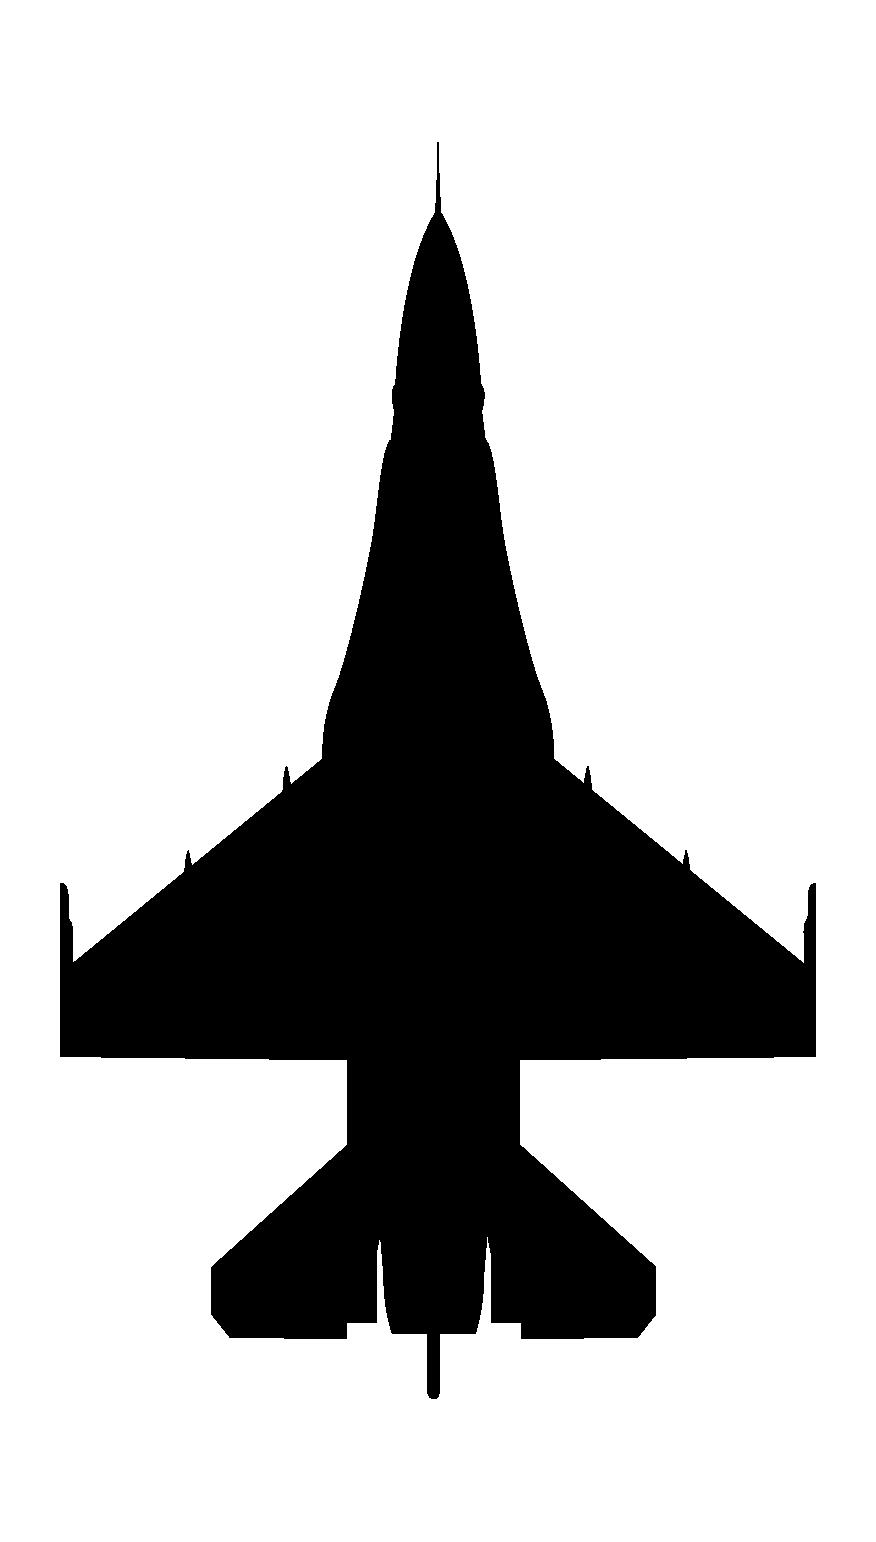
\includegraphics[
                height=15mm,
                angle=-90,
            ]{diagrams/aircraft/silhouette_f16_top.pdf}
        };

        \coordinate (offset) at (-3.5,0);
        \coordinate (center) at ($(offset)+(0:38)$);

        \draw[]
        (offset) -- node[pos=1, above right, font=\small\bfseries] {A6} +(60:30) arc (60:-60:30) -- cycle;
        \draw[]
        (offset) -- node[pos=1, above right, font=\small\bfseries] {A3} +(30:32) arc (30:-30:32) -- cycle;
        \draw[]
        (offset) -- +(25:34) arc (25:-25:34) -- node[pos=0, right, font=\small\bfseries] {A2} cycle;
        \draw[]
        (offset) -- node[pos=1, right, font=\small\bfseries] {A1} +(10:36) arc (10:-10:36) -- cycle;
        \draw[color2, fill=color2!20]
        (offset) -- +(1.5:38) arc (1.5:-1.5:38) -- cycle;

        \node[anchor=west, align=left, font=\small\bfseries, color2] at (center) {BEAMWIDTH};
    \end{tikzpicture}
    \caption{
        FCR azimuth scan \& limits. 
        Note that the A6 pattern scans the entire azimuth range of the radar.
        The varying radii for the different azimuth settings are for illustrative purposes.
    }
    \label{fig:sensors_aa:apg68:crm:azscan}
\end{figure}

\begin{figure}[htbp]
    \centering
    \begin{tikzpicture}[auto, node distance=10mm, x=1mm, y=1mm, very thick, line cap=round,
        >={Latex[round]}
        ]

        \node[
            anchor=east
        ] (mfd) at (0,0) {
            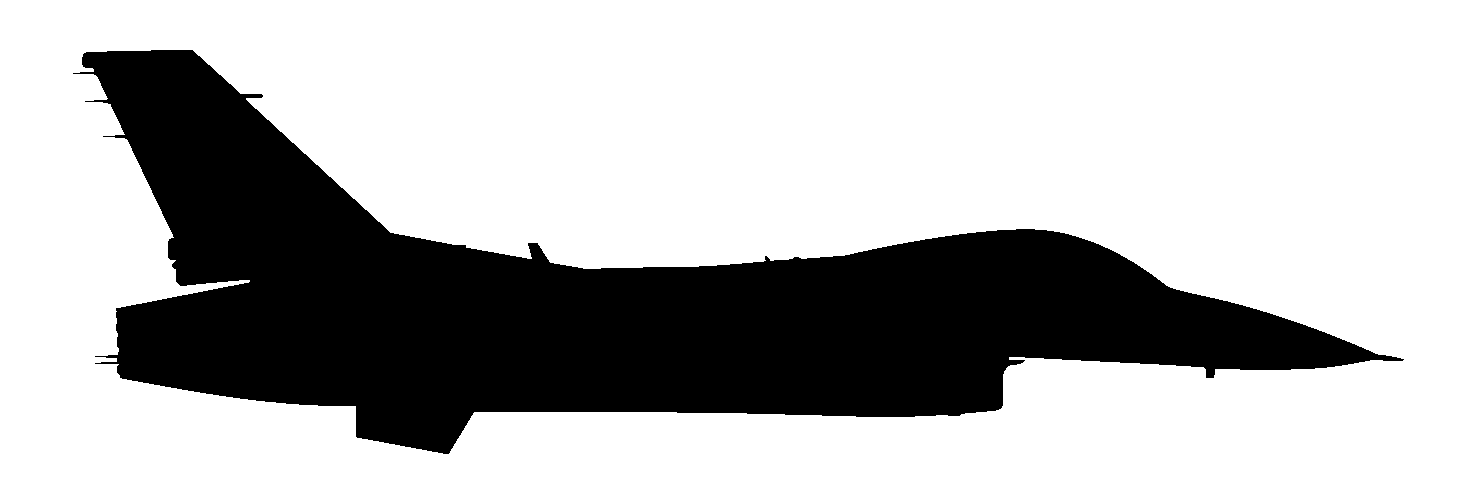
\includegraphics[
                width=15mm,
            ]{diagrams/aircraft/silhouette_f16_side.pdf}
        };

        \coordinate (offset) at (-2.5,-1);
        \coordinate (4bar) at ($(offset) + (36:35)$);
        \coordinate (3bar) at ($(offset) + (12:35)$);
        \coordinate (2bar) at ($(offset) + (-12:35)$);
        \coordinate (1bar) at ($(offset) + (-36:35)$);

        \node[font=\small\bfseries] at ($(4bar)+(5,2.5)$) {4B};
        \node[font=\small\bfseries] at ($(3bar)+(5,0)$) {3B};
        \node[font=\small\bfseries] at ($(2bar)+(5,0)$) {2B};
        \node[font=\small\bfseries] at ($(1bar)+(5,-2.5)$) {1B};

        \draw[]
        (offset) -- node[pos=1, above, font=\small\bfseries] {+/- 60 deg} +(60:35) arc (60:-60:35) -- cycle;
        \draw[color2, fill=color2!20]
        (offset) -- +(41.75:35) arc (41.75:31.25:35) -- cycle;
        \draw[color2, fill=color2!20]
        (offset) -- +(16.65:35) arc (16.65:7.35:35) -- cycle;
        \draw[color2, fill=color2!20]
        (offset) -- +(-8.45:35) arc (-8.45:-15.55:35) -- cycle;
        \draw[color2, fill=color2!20]
        (offset) -- +(-33.55:35) arc (-33.55:-38.45:35) -- cycle;

        \coordinate (4boffset) at ($(4bar) + (15,2.5)$);
        \coordinate (3boffset) at ($(3bar) + (15,0)$);
        \coordinate (2boffset) at ($(2bar) + (15,0)$);
        \coordinate (1boffset) at ($(1bar) + (15,-2.5)$);

        % 4bar
        \filldraw[color2!20] ($(4boffset) + (22.5,3.75)$) circle (2.5);

        \draw[->, rounded corners, ultra thick,]
        (4boffset)
        -- ($(4boffset) + (0,3.75)$)  -- ($(4boffset) + (20,3.75)$);
        \draw[->, rounded corners, ultra thick,]
        ($(4boffset) + (20,3.75)$)
        -- ($(4boffset) + (40,3.75)$) -- ++(0,-2.5)
        -- ++(-39,0) -- ++(0, -2.5)
        -- ++(39,0) -- ($(4boffset) + (+40,-3.75)$)
        -- ($(4boffset) + (20,-3.75)$);
        \draw[rounded corners, ultra thick,]
        ($(4boffset) + (20,-3.75)$)
        -- ($(4boffset) + (0,-3.75)$) 
        -- (4boffset);

        \draw[dashed, rounded corners=5]
        ($(4boffset) + (-2.5,6.25)$) -- ($(4boffset) + (42.5,6.25)$)
        -- ($(4boffset) + (42.5,-6.25)$) -- ($(4boffset) + (-2.5,-6.25)$)
        -- cycle;

        \draw[color2, ultra thick] ($(4boffset) + (22.5,3.75)$) circle (2.5);

        % 3bar
        \draw[->, rounded corners, ultra thick,]
        ($(3boffset) + (2.5,0)$) -- (3boffset)
        -- ($(3boffset) + (0,2.5)$) -- ($(3boffset) + (20,2.5)$);
        \draw[->, rounded corners, ultra thick,]
        ($(3boffset) + (20,2.5)$)
        -- ($(3boffset) + (40,2.5)$) -- ++(0,-2.5)
        -- ($(3boffset) + (20,0)$);
        \draw[->, rounded corners, ultra thick,]
        ($(3boffset) + (20,0)$)
        -- ($(3boffset) + (0,0)$) -- ++(0, -2.5)
        -- ($(3boffset) + (+20,-2.5)$);
        \draw[rounded corners, ultra thick,]
        ($(3boffset) + (+20,-2.5)$)
        -- ($(3boffset) + (+40,-2.5)$) -- ++(0,2.5)
        -- ($(3boffset) + (2.5,0)$);

        \draw[dashed, rounded corners=5]
        ($(3boffset) + (-2.5,5)$) -- ($(3boffset) + (42.5,5)$)
        -- ($(3boffset) + (42.5,-5)$) -- ($(3boffset) + (-2.5,-5)$)
        -- cycle;

        % 2bar
        \draw[->, rounded corners, ultra thick,]
        (2boffset)
        -- ($(2boffset) + (0,1.25)$) -- ($(2boffset) + (20,1.25)$);
        \draw[->, rounded corners, ultra thick,]
        ($(2boffset) + (20,1.25)$)
        -- ($(2boffset) + (40,1.25)$)
        -- ($(2boffset) + (40,-1.25)$) -- ($(2boffset) + (20,-1.25)$);
        \draw[rounded corners, ultra thick,]
        ($(2boffset) + (20,-1.25)$)
        -- ($(2boffset) + (0,-1.25)$)
        -- (2boffset);

        \draw[dashed, rounded corners=5]
        ($(2boffset) + (-2.5,3.75)$) -- ($(2boffset) + (42.5,3.75)$)
        -- ($(2boffset) + (42.5,-3.75)$) -- ($(2boffset) + (-2.5,-3.75)$)
        -- cycle;

        % 1bar
        \draw[->, rounded corners, ultra thick,]
        ($(1boffset) + (0,0)$) -- ($(1boffset) + (15,0)$);
        \draw[->, rounded corners, ultra thick,]
        ($(1boffset) + (40,0)$) -- ($(1boffset) + (25,0)$);
        \draw[rounded corners, ultra thick,]
        ($(1boffset) + (25,0)$) -- ($(1boffset) + (0,0)$);

        \draw[dashed, rounded corners=5]
        ($(1boffset) + (-2.5,2.5)$) -- ($(1boffset) + (42.5,2.5)$)
        -- ($(1boffset) + (42.5,-2.5)$) -- ($(1boffset) + (-2.5,-2.5)$)
        -- cycle;
    \end{tikzpicture}
    \caption{
        FCR elevation scan \& limits. 
        The radar beam --- blue circle --- tracks along the illustrated scan pattern in a loop, resulting in the dashed scan volume. 
        Note that the scan patterns are not drawn to scale.
    }
    \label{fig:sensors_aa:apg68:crm:barscan}
\end{figure}

\clearpage

\subsubsection{MFD CONTROLS}

\begin{tcoloritemize}
    \blueitem{Radar Mode}{
    \textbf{OSB 1} opens page allowing selection of radar mode

    \begin{subitemize}
        \item \textbf{Left Side (OSB 19-20)} --- A-A Modes
        \begin{itemize}
            \item CRM --- see \cref{subsec:crm}
            \item ACM --- see \cref{subsec:acm}
        \end{itemize}
        \item \textbf{Right Side (OSB 6-9)} --- A-G Modes
        \begin{itemize}
            \item See \cref{sec:fcr-ag}
        \end{itemize}
        \item \textbf{STBY (OSB 10)} --- places FCR in standby
    \end{subitemize}}
    \blueitem{Field of View}{
    \textbf{OSB 3} cycles field of view

    \begin{subitemize}
        \item \textbf{EXP} --- expanded field of view
        \item \textbf{NORM} --- normal field of view
    \end{subitemize}

    HOTAS \textbf{EXPAND/FOV} switch also cycles FOV}
    \blueitem{Override}{Pressing \textbf{OVRD (OSB 4)}  places FCR in standby}
    \blueitem{FCR Control}{\textbf{CNTL (OSB 5)} opens FCR control page}
    \blueitem{Datalink Mode}{\textbf{OSB 6} cycles datalink operating mode (WIP)}
    \blueitem{Declutter}{\textbf{DCLT (OSB 11)} opens FCR declutter page, allowing pilot to deselect symbology elements}
    \blueitem{Elevation Bar \break Select}{\textbf{OSB 17} cycles elevation bar search pattern}
    \blueitem{Azimuth Select}{
    \textbf{OSB 18} cycles azimuth search pattern}
    \blueitem{Range Select}{
    \textbf{OSB 19-20} adjusts FCR display range scale
    
    \begin{subitemize}
        \item \textbf{Can be cycled by ``walking'' cursor off top/bottom of display}
    \end{subitemize}
    }
\end{tcoloritemize}

\notebox{
    \textbf{Azimuth and range can also be cycled by ``walking'' acquisition cursor of side of FCR display}
}

\begin{figure}[htbp]
    \centering
    \begin{tikzpicture}[auto, node distance=10mm, x=1mm, y=1mm, very thick, line cap=round,
        >={Latex[round]}
        ]
        
        \node[] (fig) at (0,0) {
            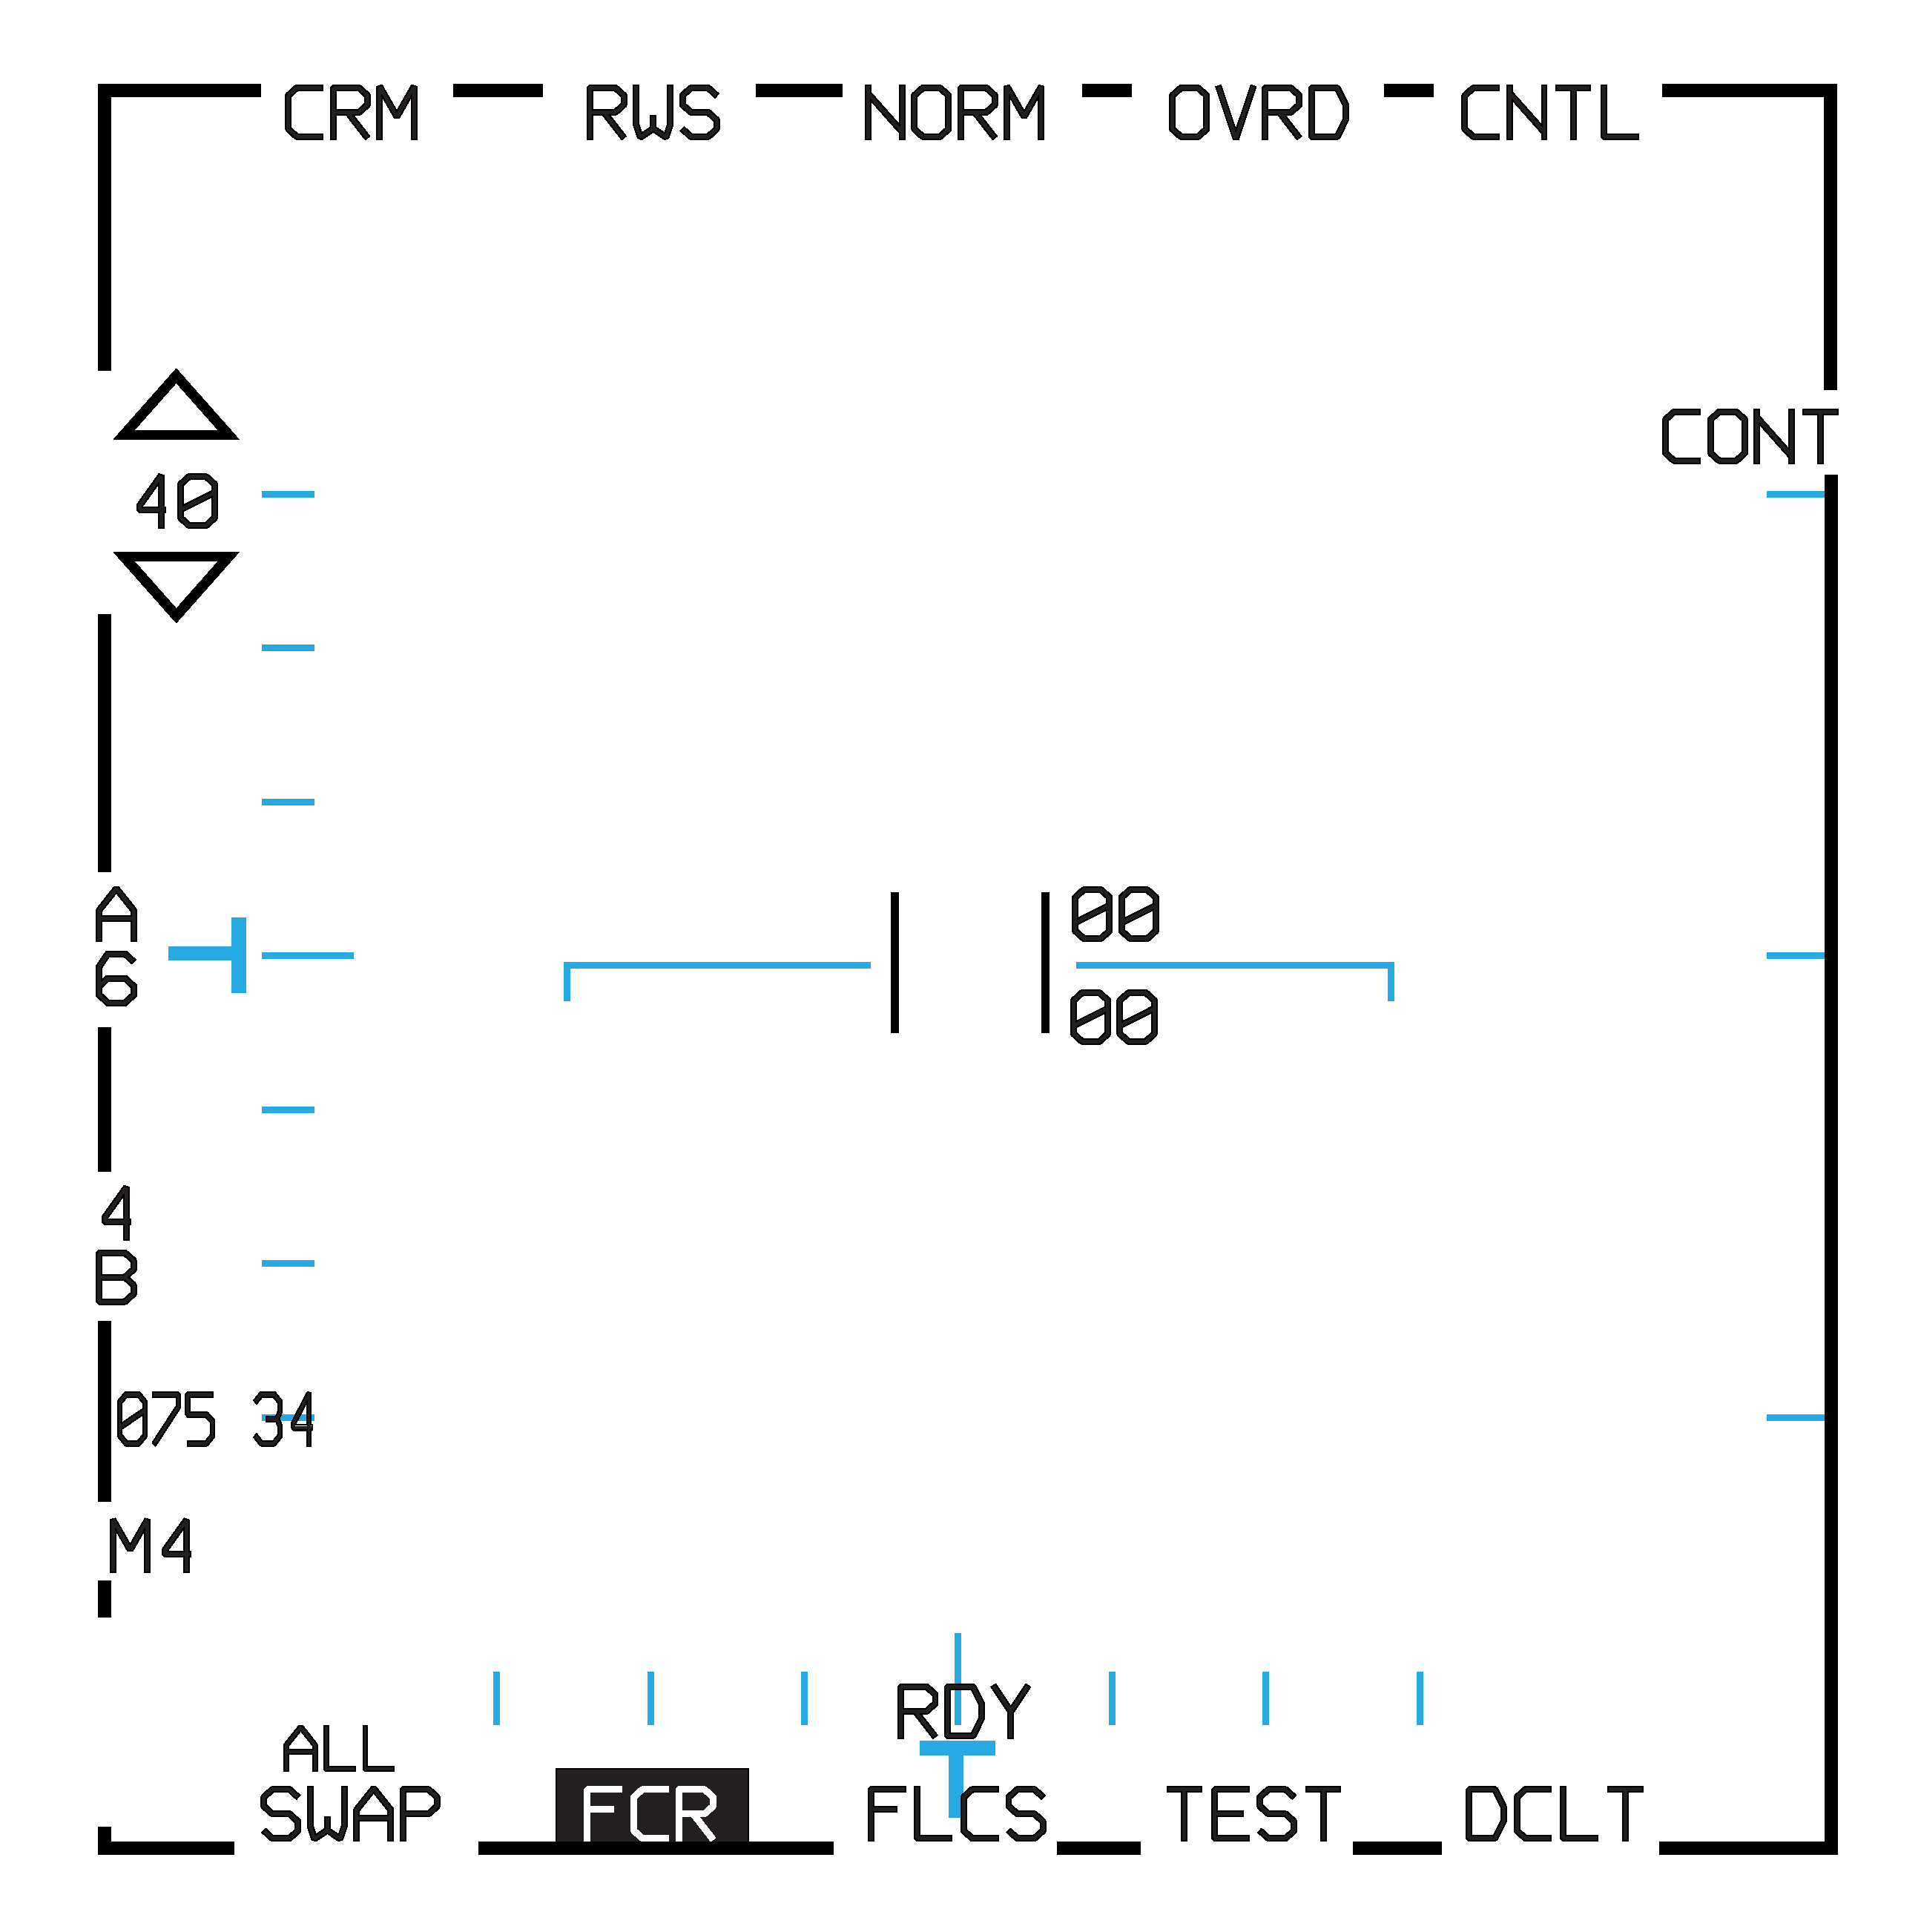
\includegraphics[
                height=75mm,
            ]{mfd/fcr_aa/rws_homepage.pdf}
        };

        % Annotations
        \node[lannot] (mode) at ($(fig.west)+(0mm,38mm)$) {FCR mode};
        \draw[->, red] (mode.east) -- ++(12mm, 0mm) -- (-24mm,35mm);

        \node[lannot] (submode) at ($(fig.west)+(0mm,28mm)$) {CRM \\ submode};
        \draw[->, red] (submode.east) -- ++(23mm, 0mm) -- (-13mm, 31mm);

        \node[lannot] (rsel) at ($(fig.west)+(0mm,18mm)$) {Range select};
        \draw[->, red] (rsel.east) -- ++(4.5mm, 0mm);

        \node[lannot] (asel) at ($(fig.west)+(0mm,0.5mm)$) {Azimuth select};
        \draw[->, red] (asel.east) -- ++(4.5mm, 0mm);

        \node[lannot] (bsel) at ($(fig.west)+(0mm,-10.5mm)$) {Elevation bar select};
        \draw[->, red] (bsel.east) -- ++(4.5mm, 0mm);

        \node[annot, anchor=south, align=center] (fov) at ($(fig.north)+(0mm,0mm)$) {FOV select};
        \draw[->, red] (fov.south) -- ++(0mm, -3.5mm);

        \node[rannot] (cntl) at ($(fig.east)+(0mm,38mm)$) {Control};
        \draw[->, red] (cntl.west) -- ++(-13mm, 0mm) -- (23mm, 35mm);

        \node[rannot] (ovrd) at ($(fig.east)+(0mm,28mm)$) {Override};
        \draw[->, red] (ovrd.west) -- ++(-24mm, 0mm) -- (12mm, 31mm);

        \node[rannot] (dl) at ($(fig.east)+(0mm,20.5mm)$) {Datalink mode};
        \draw[->, red] (dl.west) -- ++(-4mm,0mm);

        \node[rannot] (acq) at ($(fig.east)+(0mm,10mm)$) {Acquisition cursor};
        \draw[->, red] (acq.west) -- ++(-30mm, 0mm) -- (3mm,5mm);

        \node[rannot] (sj) at ($(fig.east)+(0mm,-8mm)$) {Horizon \\indicator};
        \draw[->, red] (sj.west) -- ++(-20mm, 0mm) -- (12mm,-1mm);

        \node[rannot] (dclt) at ($(fig.east)+(0mm,-38mm)$) {Declutter};
        \draw[->, red] (dclt.west) -- ++(-13mm, 0mm) -- (23mm, -35mm);
    \end{tikzpicture}
    \caption{FCR page with basic controls \& symbology marked. Note that FCR is illustrated in default mode immediately after startup.}
\end{figure}

\clearpage

\subsection{RWS}
\label{subsec:rws}
\begin{tcoloritemize}
    \blueitem[RWS]
    \textbf{R}ange \textbf{W}hile \textbf{S}earch

    \begin{itemize}
        \item \textbf{Fast, Long(er)-Range Search}
        \begin{itemize}
            \item radar scans selectable search volume
            \item displays raw target position returns
        \end{itemize}
        \item \textbf{No track data} 
        \begin{itemize}
            \item exact target range, velocity, angle, etc.
            \item but can transition to advanced modes
        \end{itemize}
        % (exact target range, velocity, angle, etc.)
        % --- but can transition to advanced modes
    \end{itemize}
\end{tcoloritemize}

\begin{figure}[htbp]
    \centering
    \begin{tikzpicture}[auto, node distance=10mm, x=1mm, y=1mm, very thick, line cap=round,
        >={Latex[round]}
        ]
        
        \node[] (fig) at (0,0) {
            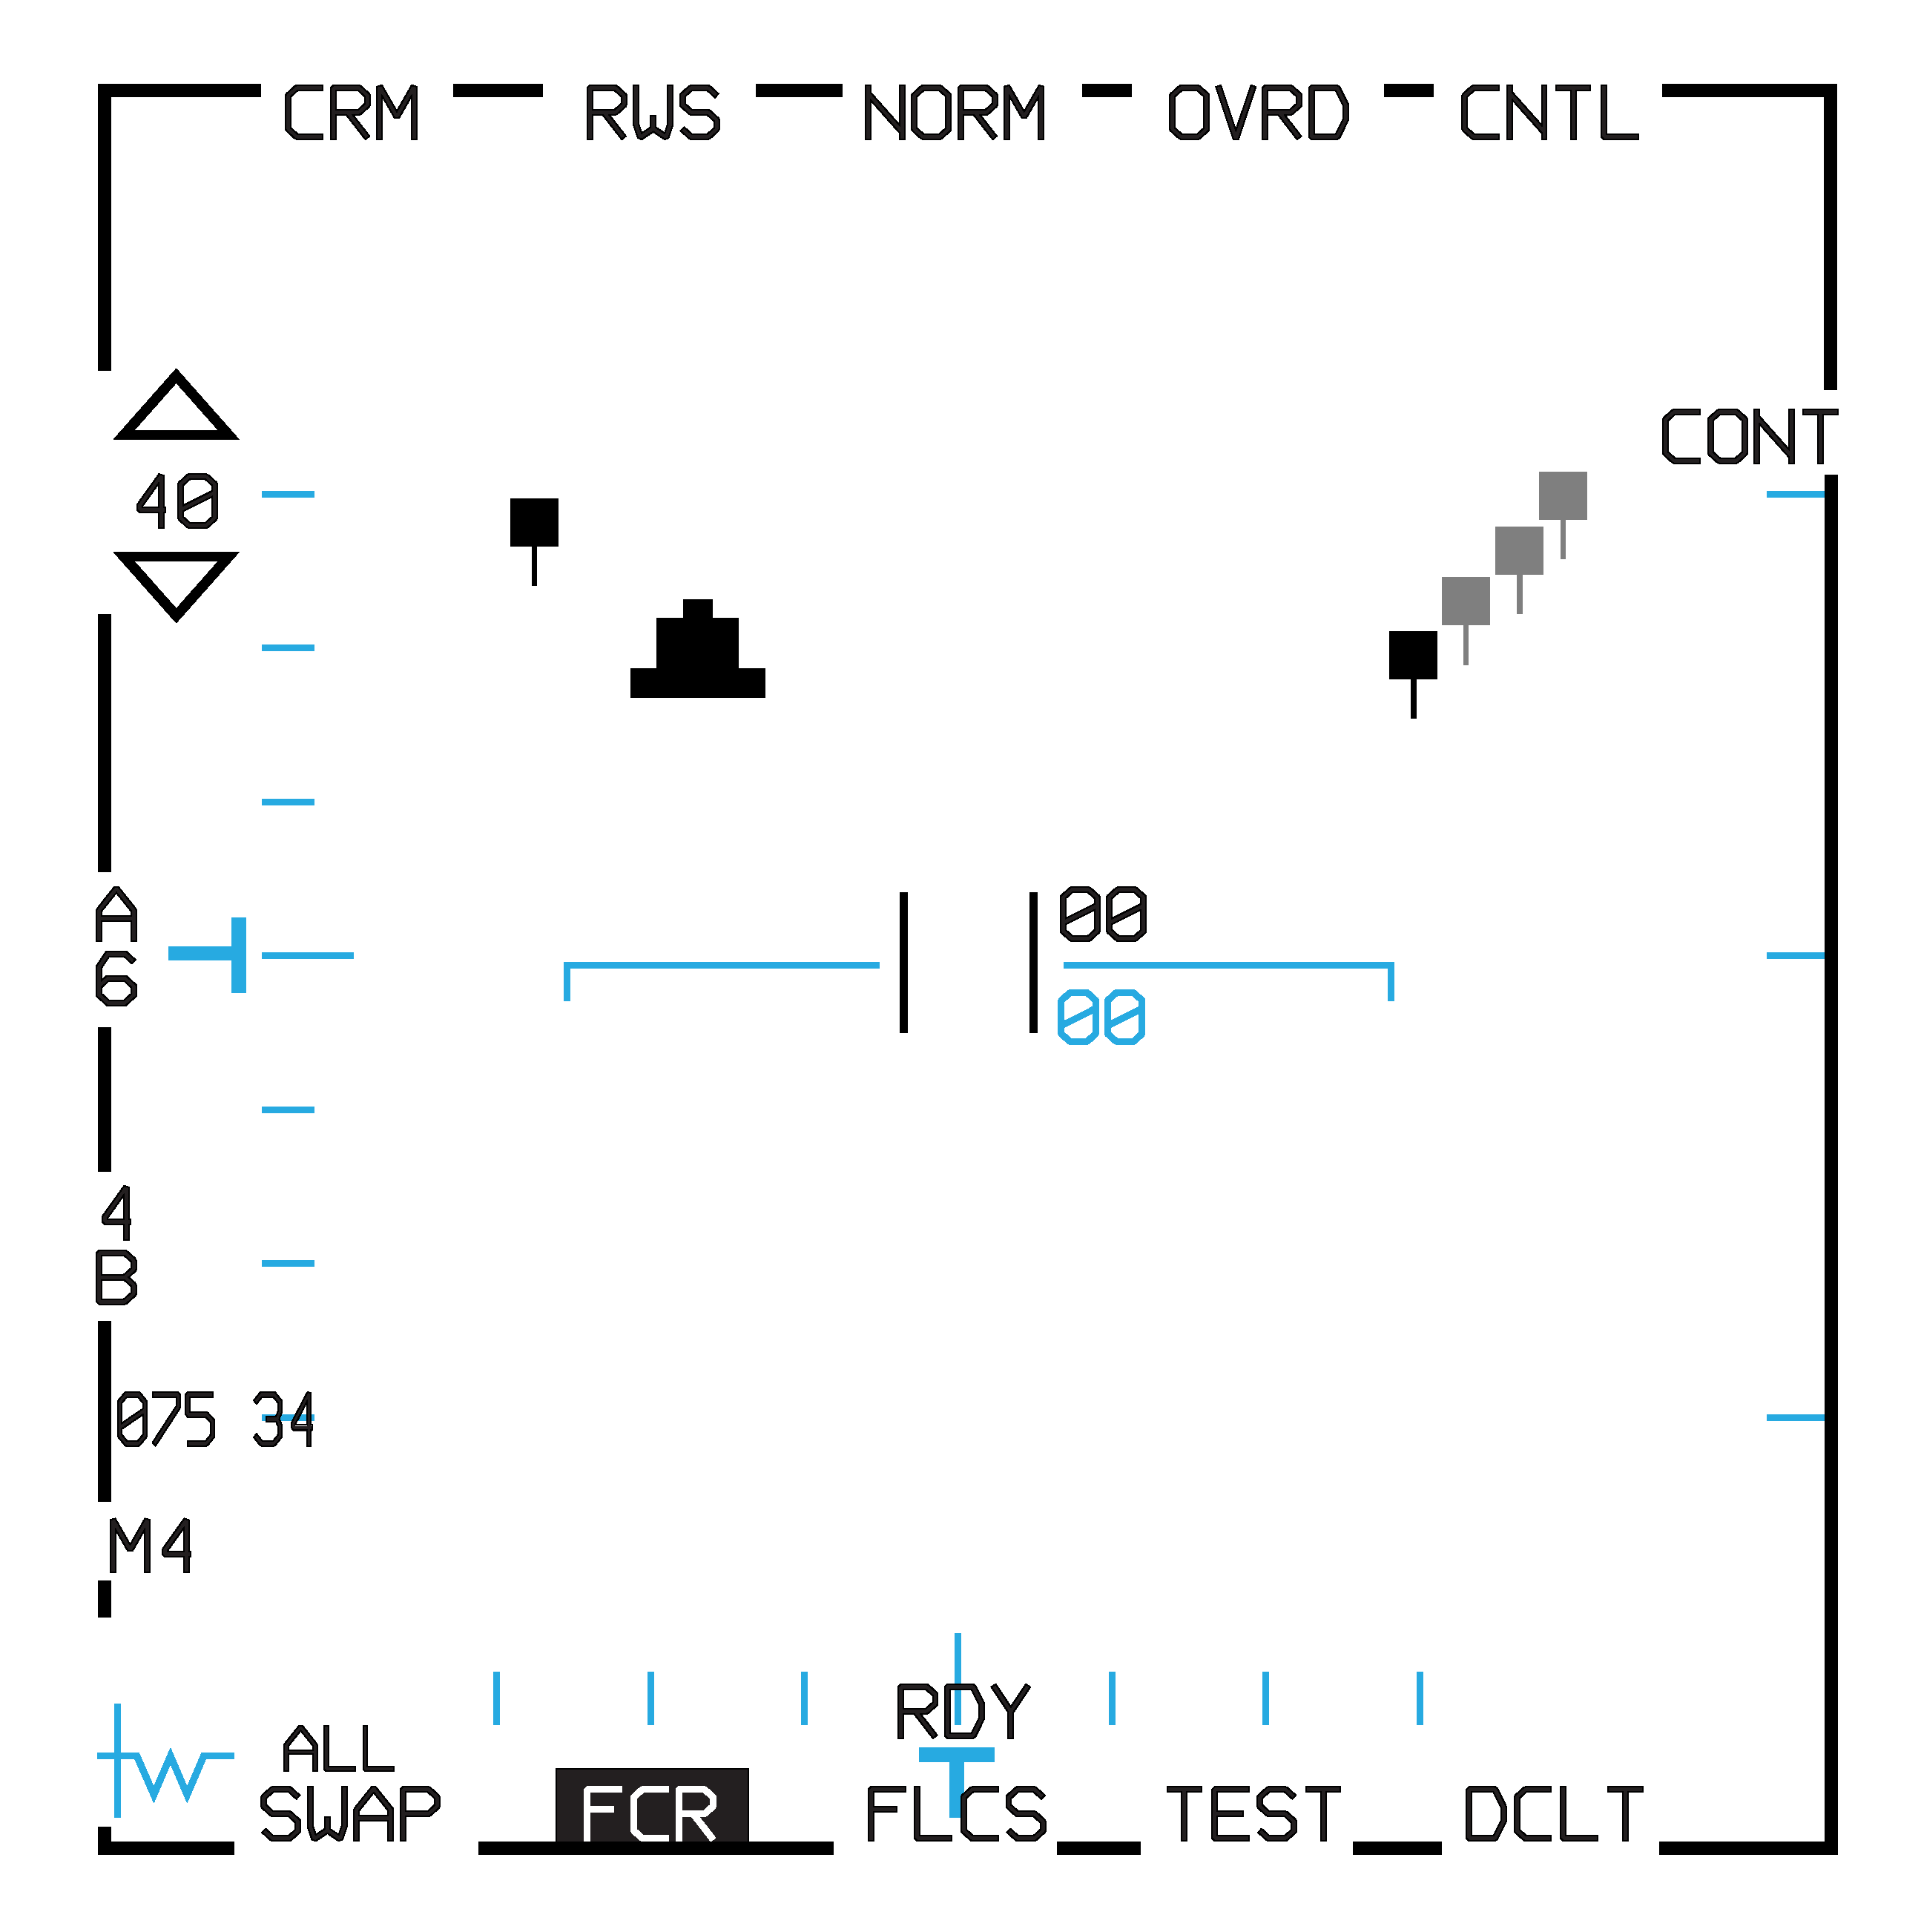
\includegraphics[
                height=75mm,
            ]{mfd/fcr_aa/rws_search.pdf}
        };

        % Annotations
        \node[lannot] (rsel) at ($(fig.west)+(0mm,18mm)$) {Range select};
        \draw[annotptr] (rsel.east) -- ++(4.5mm, 0mm);

        \node[lannot] (asel) at ($(fig.west)+(0mm,0.5mm)$) {Azimuth select};
        \draw[annotptr] (asel.east) -- ++(4.5mm, 0mm);

        \node[lannot] (bsel) at ($(fig.west)+(0mm,-10.5mm)$) {Elevation bar select};
        \draw[annotptr] (bsel.east) -- ++(4.5mm, 0mm);

        \node[rannot] (ret) at ($(fig.east)+(0mm,28mm)$) {RWS \\ returns};
        \draw[annotptr] (ret.west) -- ++(-16mm, 0mm) -- (18mm,18mm);
        \draw[annotptr] (ret.west) -- ++(-50mm, 0mm) -- (-16mm,20mm);

        \node[rannot] (stpt) at ($(fig.east)+(0mm,6mm)$) {Current STPT};
        \draw[annotptr] (stpt.west) -- ++(-42mm, 0mm) -- (-7mm,9mm);

        \node[rannot] (acq) at ($(fig.east)+(0mm,-10mm)$) {Acquisition cursor};
        \draw[annotptr] (acq.west) -- ++(-30mm, 0mm) -- (3mm,-5mm);
    \end{tikzpicture}
    \caption{RWS FCR mode symbology.}
\end{figure}

\begin{tcoloritemize}
    \blueitem[SAM \break Submode]
    \textbf{S}ituational \textbf{A}warness \textbf{M}ode

    \begin{itemize}
        \item \textbf{Target is ``Bugged''} (Pseudo-Track)
        \begin{itemize}
            \item can guide AIM-120C (w/o STT Lock)
            \item DLZ displayed if missile selected
        \end{itemize}
        \item \textbf{RWS search  continues}
        \begin{itemize}
            \item scan pauses on SAM target
            \item FCR manages scan volume
        \end{itemize}
    \end{itemize}
    \blueitem[DTT \break Submode]
    \textbf{D}ual \textbf{T}arget \textbf{T}rack

    \begin{itemize}
        \item \textbf{2 Targets ``Bugged''} --- primary / secondary
        \begin{itemize}
            \item can guide AIM-120C on \textbf{\underline{primary target}}
            \item DLZ displayed if missile selected
        \end{itemize}
        \item \textbf{TMS Left --- swaps primary / secondary}
        \item \textbf{RWS search  continues}
        \begin{itemize}
            \item scan pauses on both primary / secondary
            \item FCR manages scan volume
        \end{itemize}
        \item \textbf{Within 10nm search pattern inhibited} --- radar only scans primary/secondary targets
        \item \textbf{Once \underline{either} target within 3nm automatically transitions to STT}
    \end{itemize}
    \blueitem[Spotlight]
        
    \textbf{Narrow scan centered on acquisition cursor}
    \begin{itemize}
        \item \textbf{Narrow scan}
        \begin{itemize}
            \item 4 bar elevation 
            \item \pm10 deg azimuth
        \end{itemize}
        \item Useful to rapidly acquire radar returns from target at known position
        \item \textbf{Activated by holding TMS Forward >1 sec}
        \begin{itemize}
            \item enters SAM submode if target detected under Acquisition Cursor
            \item returns to previous search pattern if no target under Acquisition Cursor when released
        \end{itemize}
    \end{itemize}
\end{tcoloritemize}

\begin{figure}[htbp]
    \centering
    \begin{tikzpicture}[auto, node distance=10mm, x=1mm, y=1mm, very thick, line cap=round,
        >={Latex[round]}
        ]
        
        \node[] (fig) at (0,0) {
            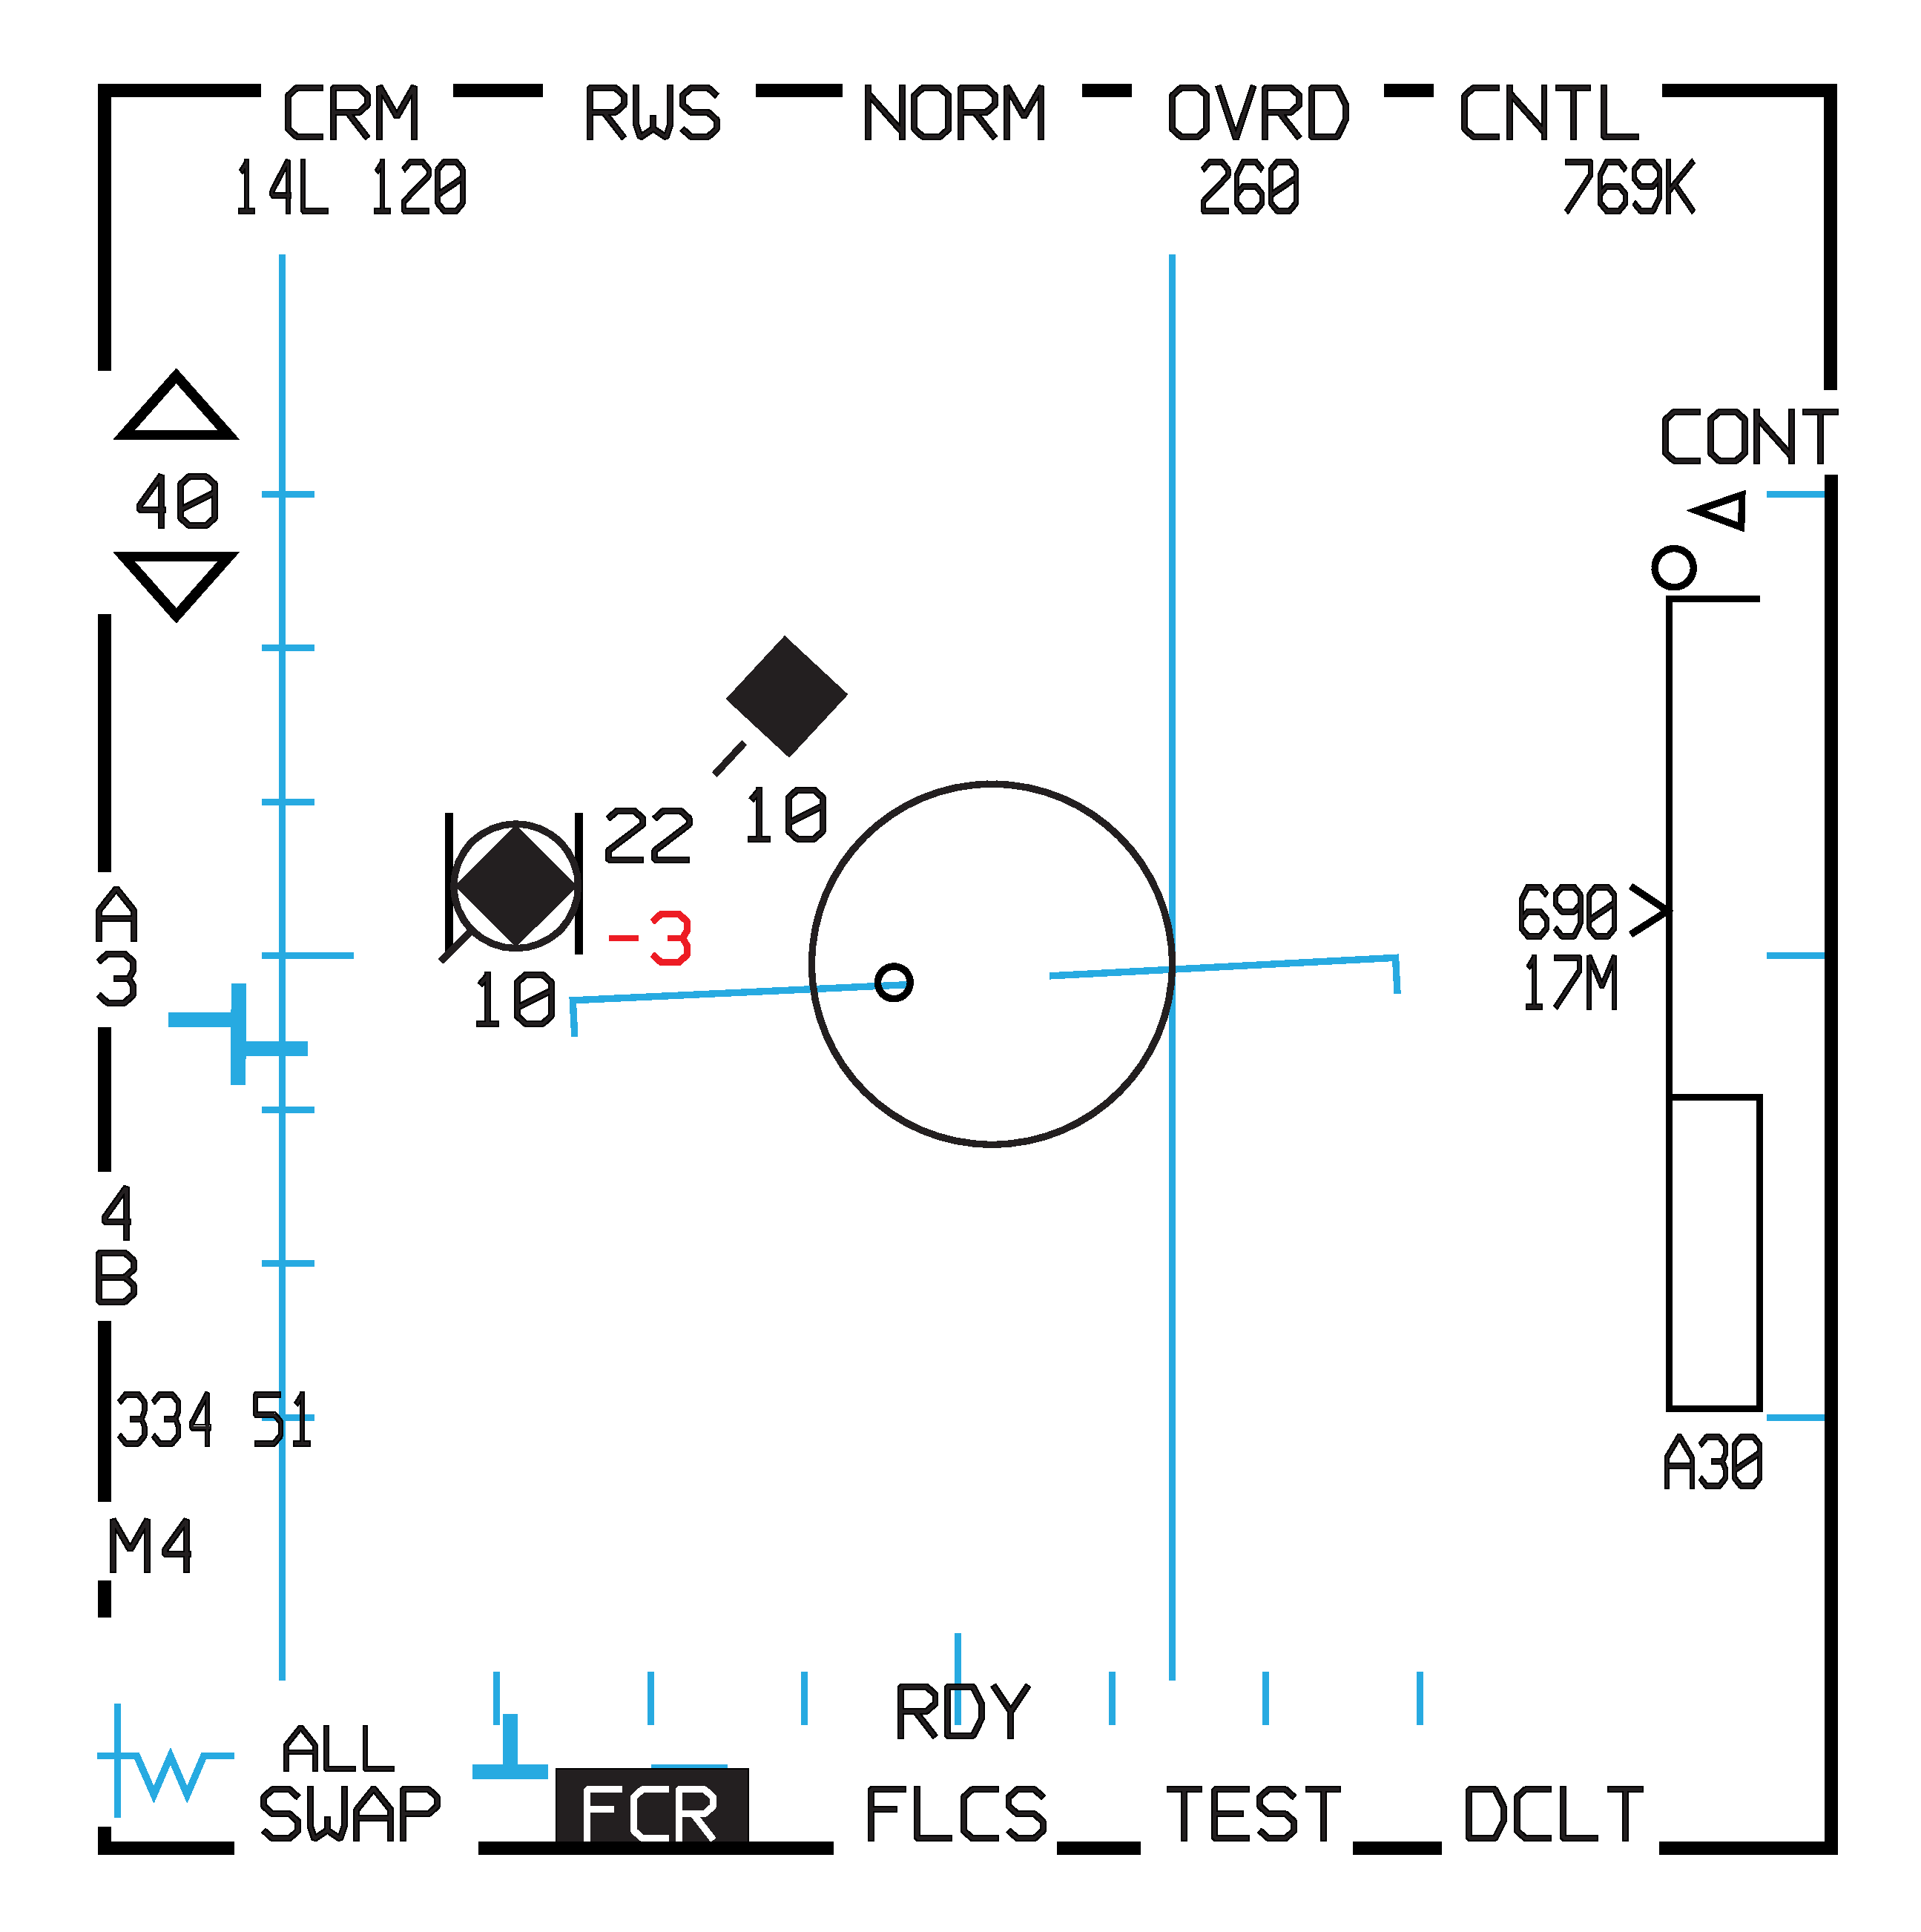
\includegraphics[
                height=75mm,
            ]{mfd/fcr_aa/rws_sam_dtt.pdf}
        };

        % Annotations
        \node[lannot] (asp) at ($(fig.west)+(0mm,30.25mm)$) {Aspect};
        \draw[annotptr] (asp.east) -- ++(9mm, 0mm);

        \node[lannot] (trk) at ($(fig.west)+(0mm,24mm)$) {Track};
        \draw[annotptr] (trk.east) -- ++(12mm, 0mm) -- ++(4mm, 4mm);

        \node[lannot] (sec) at ($(fig.west)+(0mm,10.25mm)$) {Secondary target};
        \draw[annotptr] (sec.east) -- ++(27mm, 0mm);

        \node[lannot] (prim) at ($(fig.west)+(0mm,-7mm)$) {Primary target \& cursor};
        \draw[annotptr] (prim.east) -- ++(15mm, 0mm) -- ++(4mm, 6mm);

        \node[rannot] (clos) at ($(fig.east)+(0mm,30.25mm)$) {Closure};
        \draw[annotptr] (clos.west) -- ++(-9mm, 0mm);

        \node[rannot] (as) at ($(fig.east)+(0mm,24mm)$) {Airspeed};
        \draw[annotptr] (as.west) -- ++(-22mm, 0mm) -- ++(-4mm, 4mm);

        \node[rannot] (dlz) at ($(fig.east)+(0mm,-2mm)$) {DLZ \\ {\footnotesize see \cref{fig:aa_weap:aim120:dlz}}};
        \draw[annotptr] (dlz.west) -- ++(-8mm, 0mm);

        \node[rannot] (asec) at ($(fig.east)+(0mm,-24mm)$) {ASC / ASEC \\ {\footnotesize see \cref{fig:aa_weap:aim120:asc_asec}}};
        \draw[annotptr] (asec.west) -- ++(-26mm, 0mm) -- (4mm,-7mm);

        \node[annot, anchor=south, align=left, text width=35mm] (fov) at ($(fig.north)+(-6.5mm,0mm)$) {Azimuth scan limits};
        \draw[annotptr] (fov.south) -- ++(0mm, -15mm) -- ++(12mm, -6mm);
    \end{tikzpicture}
    \caption{RWS SAM / DTT submode symbology. Additional information on primary target is displayed at top of FCR page.}
\end{figure}

\marginfigeometry

\subsubsection{SELECT RWS MODE}
\begin{checklistenumerate}
    \blueitem[FCR Switch] \textbf{FCR}
    \blueitem[Desired MFD] \textbf{FCR Page}, verify \textbf{SOI}
    \blueitem[Radar Mode]
        \textbf{CRM} (default), verify

        \begin{itemize}
            \item \textbf{Dogfight/Missile Override} --- \textbf{NORM}
            \item \textbf{Radar Mode (OSB 1)} --- shows \textbf{CRM}
        \end{itemize}
    \blueitem[CRM Submode]
        \textbf{RWS} (default), cycle via 

        \begin{itemize}
            \item \textbf{TMS Right (long)} / \textbf{OSB 2} 
        \end{itemize}
\end{checklistenumerate}

\subsubsection{SAM / DTT ACQUISITION}
\label{subsec:rws:samdttacq}
\begin{checklistenumerate}
    \blueitem[Locate Targets]
    \begin{enumerate}
        \item Correlate onboard/offboard sensors
        \begin{itemize}
            \item raw radar returns, RWR pings
            \item AWACS calls, datalink targets
        \end{itemize}
        \item Place targets within radar scan volume
    \end{enumerate}
    \blueitem[SAM Acquisition]
    \marginpar{
        \captionsetup{type=figure}
        \centering
        \begin{tikzpicture}[figstyle]
            
            \node[boxedmarfigstyle] (search) at (0,0) {
                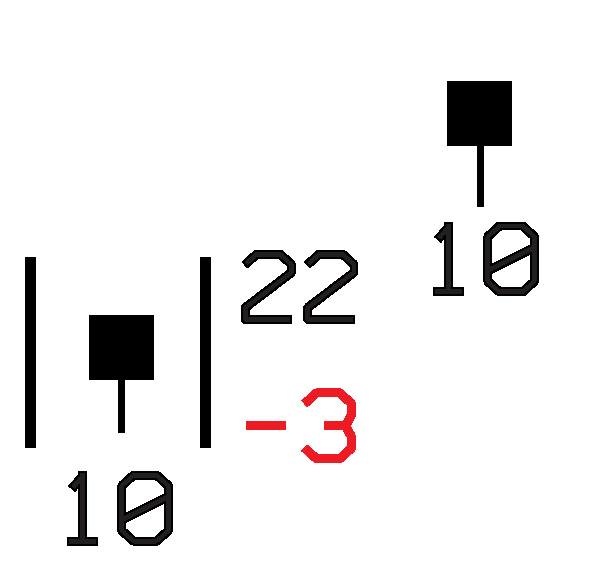
\includegraphics[
                    scale=0.25,
                ]{mfd/fcr_aa/rws_sam_dtt_subfig_01.pdf}
            };
            \node[boxedmarfigstyle] (sam) at (0,-35) {
                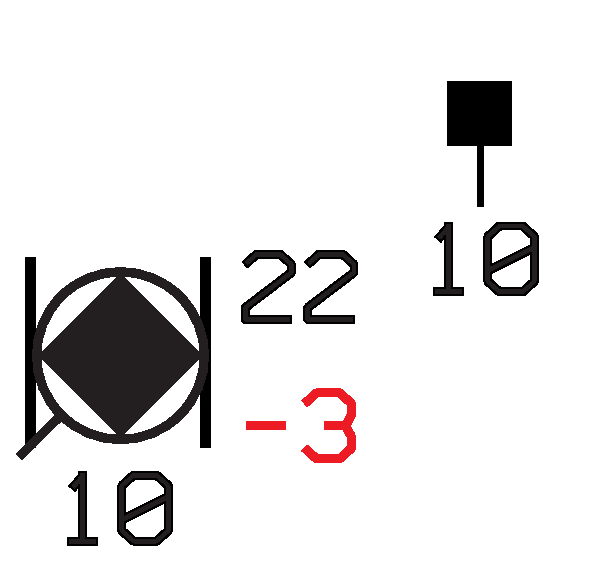
\includegraphics[
                    scale=0.25,
                ]{mfd/fcr_aa/rws_sam_dtt_subfig_02.pdf}
            };

            \draw[->]
            (search) -- node[right, align=center, font=\small] {\textbf{TMS} \textbf{FWD}}(sam);
        \end{tikzpicture}
        \caption{SAM Acquisition}
    }
    \begin{enumerate}
        \item \textbf{Target} \dotfill under Acquisition Cursor
        \item \textbf{TMS} \dotfill \textbf{Forward (hold)}
        \item \textbf{Target} \dotfill Verify \textbf{Bugged}
    \end{enumerate}
    \begin{itemize}
        \item Can guide AIM-120C on Bugged target
        \item DLZ displayed if missile selected
        \item RWS search continues
    \end{itemize}
    \blueitem[DTT Acquisition] (if desired)
    \marginpar{
        \captionsetup{type=figure}
        \centering
        \begin{tikzpicture}[figstyle]
            
            \node[boxedmarfigstyle] (sam) at (0,0) {
                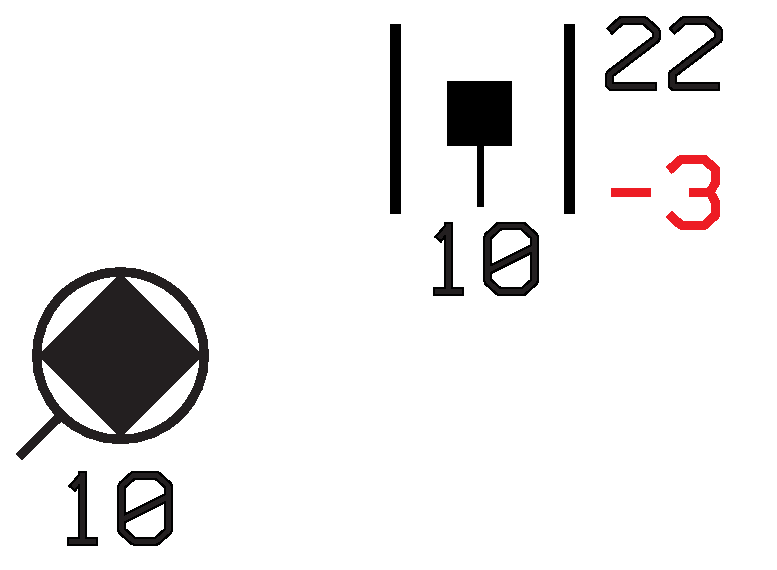
\includegraphics[
                    scale=0.25,
                ]{mfd/fcr_aa/rws_sam_dtt_subfig_03.pdf}
            };
            \node[boxedmarfigstyle] (dtt) at (0,-35) {
                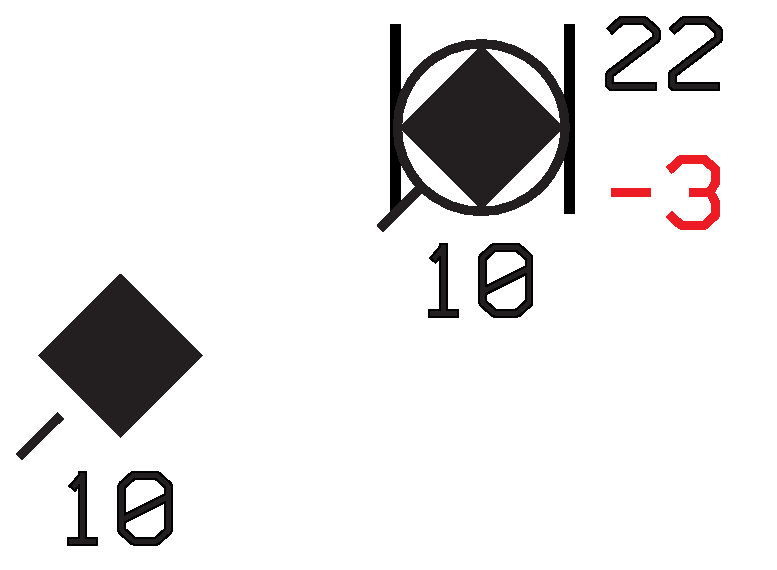
\includegraphics[
                    scale=0.25,
                ]{mfd/fcr_aa/rws_sam_dtt_subfig_04.pdf}
            };

            \draw[->]
            (sam) -- node[right, align=center, font=\small] {\textbf{TMS} \textbf{FWD}}(dtt);
        \end{tikzpicture}
        \caption{DTT Acquisition}
    }
    \begin{enumerate}
        \item \textbf{Target 2} \dotfill under Acquisition Cursor
        \item \textbf{TMS} \dotfill \textbf{Forward (hold)}
    \end{enumerate}

    To swap primary / secondary target

    \begin{enumerate}[start=3]
        \item \textbf{TMS} \dotfill \textbf{Left}
    \end{enumerate}
    \blueitem[STT Lock] (if desired)
    \begin{enumerate}
        \item \textbf{Target} \dotfill under Acquisition Cursor
        \item \textbf{TMS} \dotfill \textbf{Forward}
    \end{enumerate}
\end{checklistenumerate}

\subsubsection{SPOTLIGHT ACQUISITION}
\begin{checklistenumerate}
    \blueitem[Locate Targets]
    \begin{enumerate}
        \item Correlate onboard/offboard sensors
        \begin{itemize}
            \item raw radar returns, RWR pings
            \item AWACS calls, datalink targets
        \end{itemize}
        \item Place target within radar scan limits
    \end{enumerate}
    \blueitem[Spotlight Search]
    \marginpar{
        \captionsetup{type=figure}
        \centering
        \begin{tikzpicture}[figstyle]
            
            \node[
                boxedmarfigstyle,            
            ] (cursoroff) at (0,0) {
                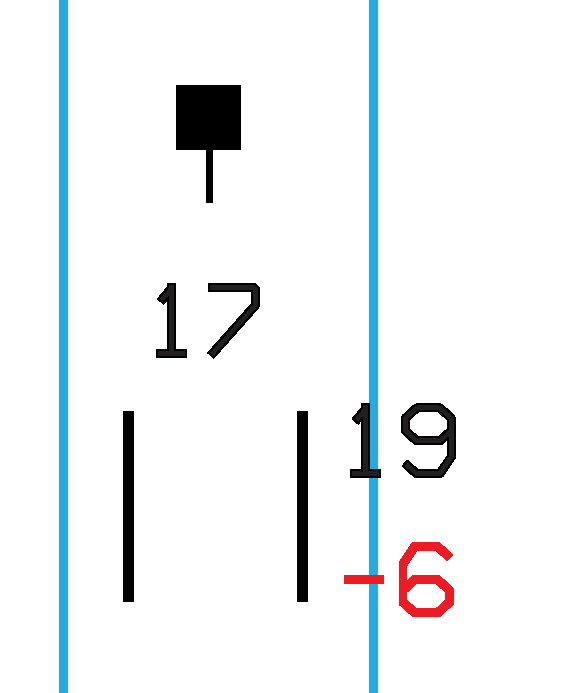
\includegraphics[
                    scale=0.25,
                ]{mfd/fcr_aa/rws_spotlight_subfig_cursor_off.pdf}
            };
            \node[
                boxedmarfigstyle,                
                below=10 of cursoroff,
            ] (cursoron) {
                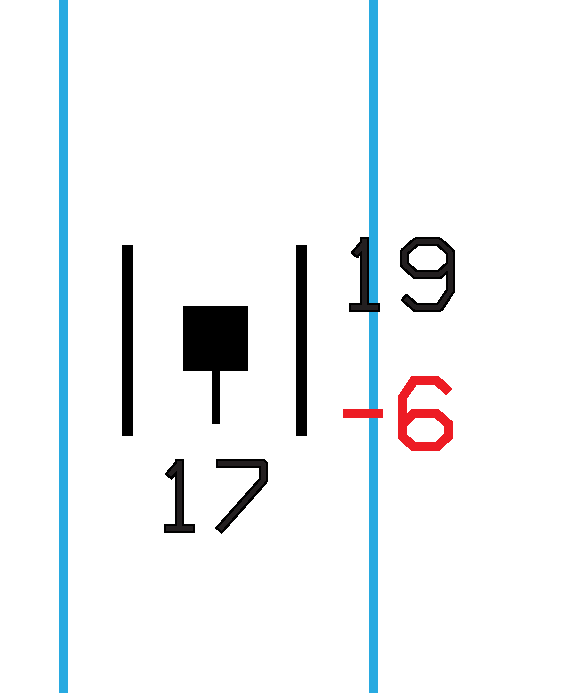
\includegraphics[
                    scale=0.25,
                ]{mfd/fcr_aa/rws_spotlight_subfig_cursor_on.pdf}
            };
            \node[
                boxedmarfigstyle,                
                below=10 of cursoron,
            ] (bugged) {
                
\includegraphics[
                    scale=0.5,
                ]{mfd/fcr_aa/tgt_bugged.pdf}
            };

            % lines
            \draw[->]
            ($(cursoroff.north) + (0,5)$) -- node[pos=0, above, align=left, font=\small] {\textbf{TMS} \textbf{FWD (hold)}}(cursoroff);
            \draw[->]
            (cursoroff) -- node[right, align=left, font=\small] {\textbf{Slew over} \\ \textbf{target}}(cursoron);
            \draw[->]
            (cursoron) -- node[right, align=left, font=\small] {\textbf{TMS FWD} \\ \textbf{(release)}}(bugged);

            % labels
            \node[
                anchor=north west,
                align=left,
                font=\bfseries\footnotesize,
            ] (labelbugged) at (bugged.north west) {Bugged \\ Target};
        \end{tikzpicture}
        \caption{Spotlight Search}
    }
    \begin{enumerate}
        \item \textbf{Target} \dotfill near Acquisition Cursor
        \item \textbf{TMS} \dotfill \textbf{Forward (hold)}
        \begin{itemize}
            \item FCR enters \pm10deg scan around acquisition cursor
        \end{itemize}
    \end{enumerate}
    \blueitem[SAM Acquisition]
    \begin{enumerate}
        \item \textbf{Target} \dotfill under Acquisition Cursor
        \item \textbf{TMS} \dotfill \textbf{Forward (release)}
        \item \textbf{Target} \dotfill Verify \textbf{Bugged}
    \end{enumerate}
    \begin{itemize}
        \item Can guide AIM-120C on Bugged target
        \item DLZ displayed if missile selected
        \item RWS search continues
    \end{itemize}
    \blueitem[STT Lock] (if desired)
    \begin{enumerate}
        \item \textbf{Target} \dotfill under Acquisition Cursor
        \item \textbf{TMS} \dotfill \textbf{Forward}
    \end{enumerate}
\end{checklistenumerate}

\marginfigrestore

\clearpage

\subsection{TWS}
\label{subsec:tws}
\begin{tcoloritemize}
    \blueitem[TWS]
    \textbf{T}rack \textbf{W}hile \textbf{S}can --- reference \cref{fig:sensors_aa:apg68:tws:search} for symbology

    \begin{itemize}
        \item \textbf{Multi-target tracking mode}
        \begin{itemize}
            \item allows multi-target AIM-120 engagement
            \item targets not locked --- \textbf{\underline{no RWR warning}}
        \end{itemize}
        \item \textbf{FCR builds trackfiles for each target}
        \begin{itemize}
            \item predicts target movement between scans
            \item slow update rate --- target maneuvers can cause radar to lose track
        \end{itemize}
        \item \textbf{Trackfiles can be in several states}
        \begin{itemize}
            \item search / Track / System / Cursor / Bugged
        \end{itemize}
    \end{itemize}
    
    Reference \cref{subsec:sensorsaa:apg68:tws:trackfile} for trackfile explanation \& \cref{fig:sensorsaa:apg68:tws:trackfile} for trackfile symbology
\end{tcoloritemize}

\begin{figure}[htbp]
    \centering
    \begin{tikzpicture}[auto, node distance=10mm, x=1mm, y=1mm, very thick, line cap=round,
        >={Latex[round]}
        ]
        
        \node[] (mfd) at (0,0) {
            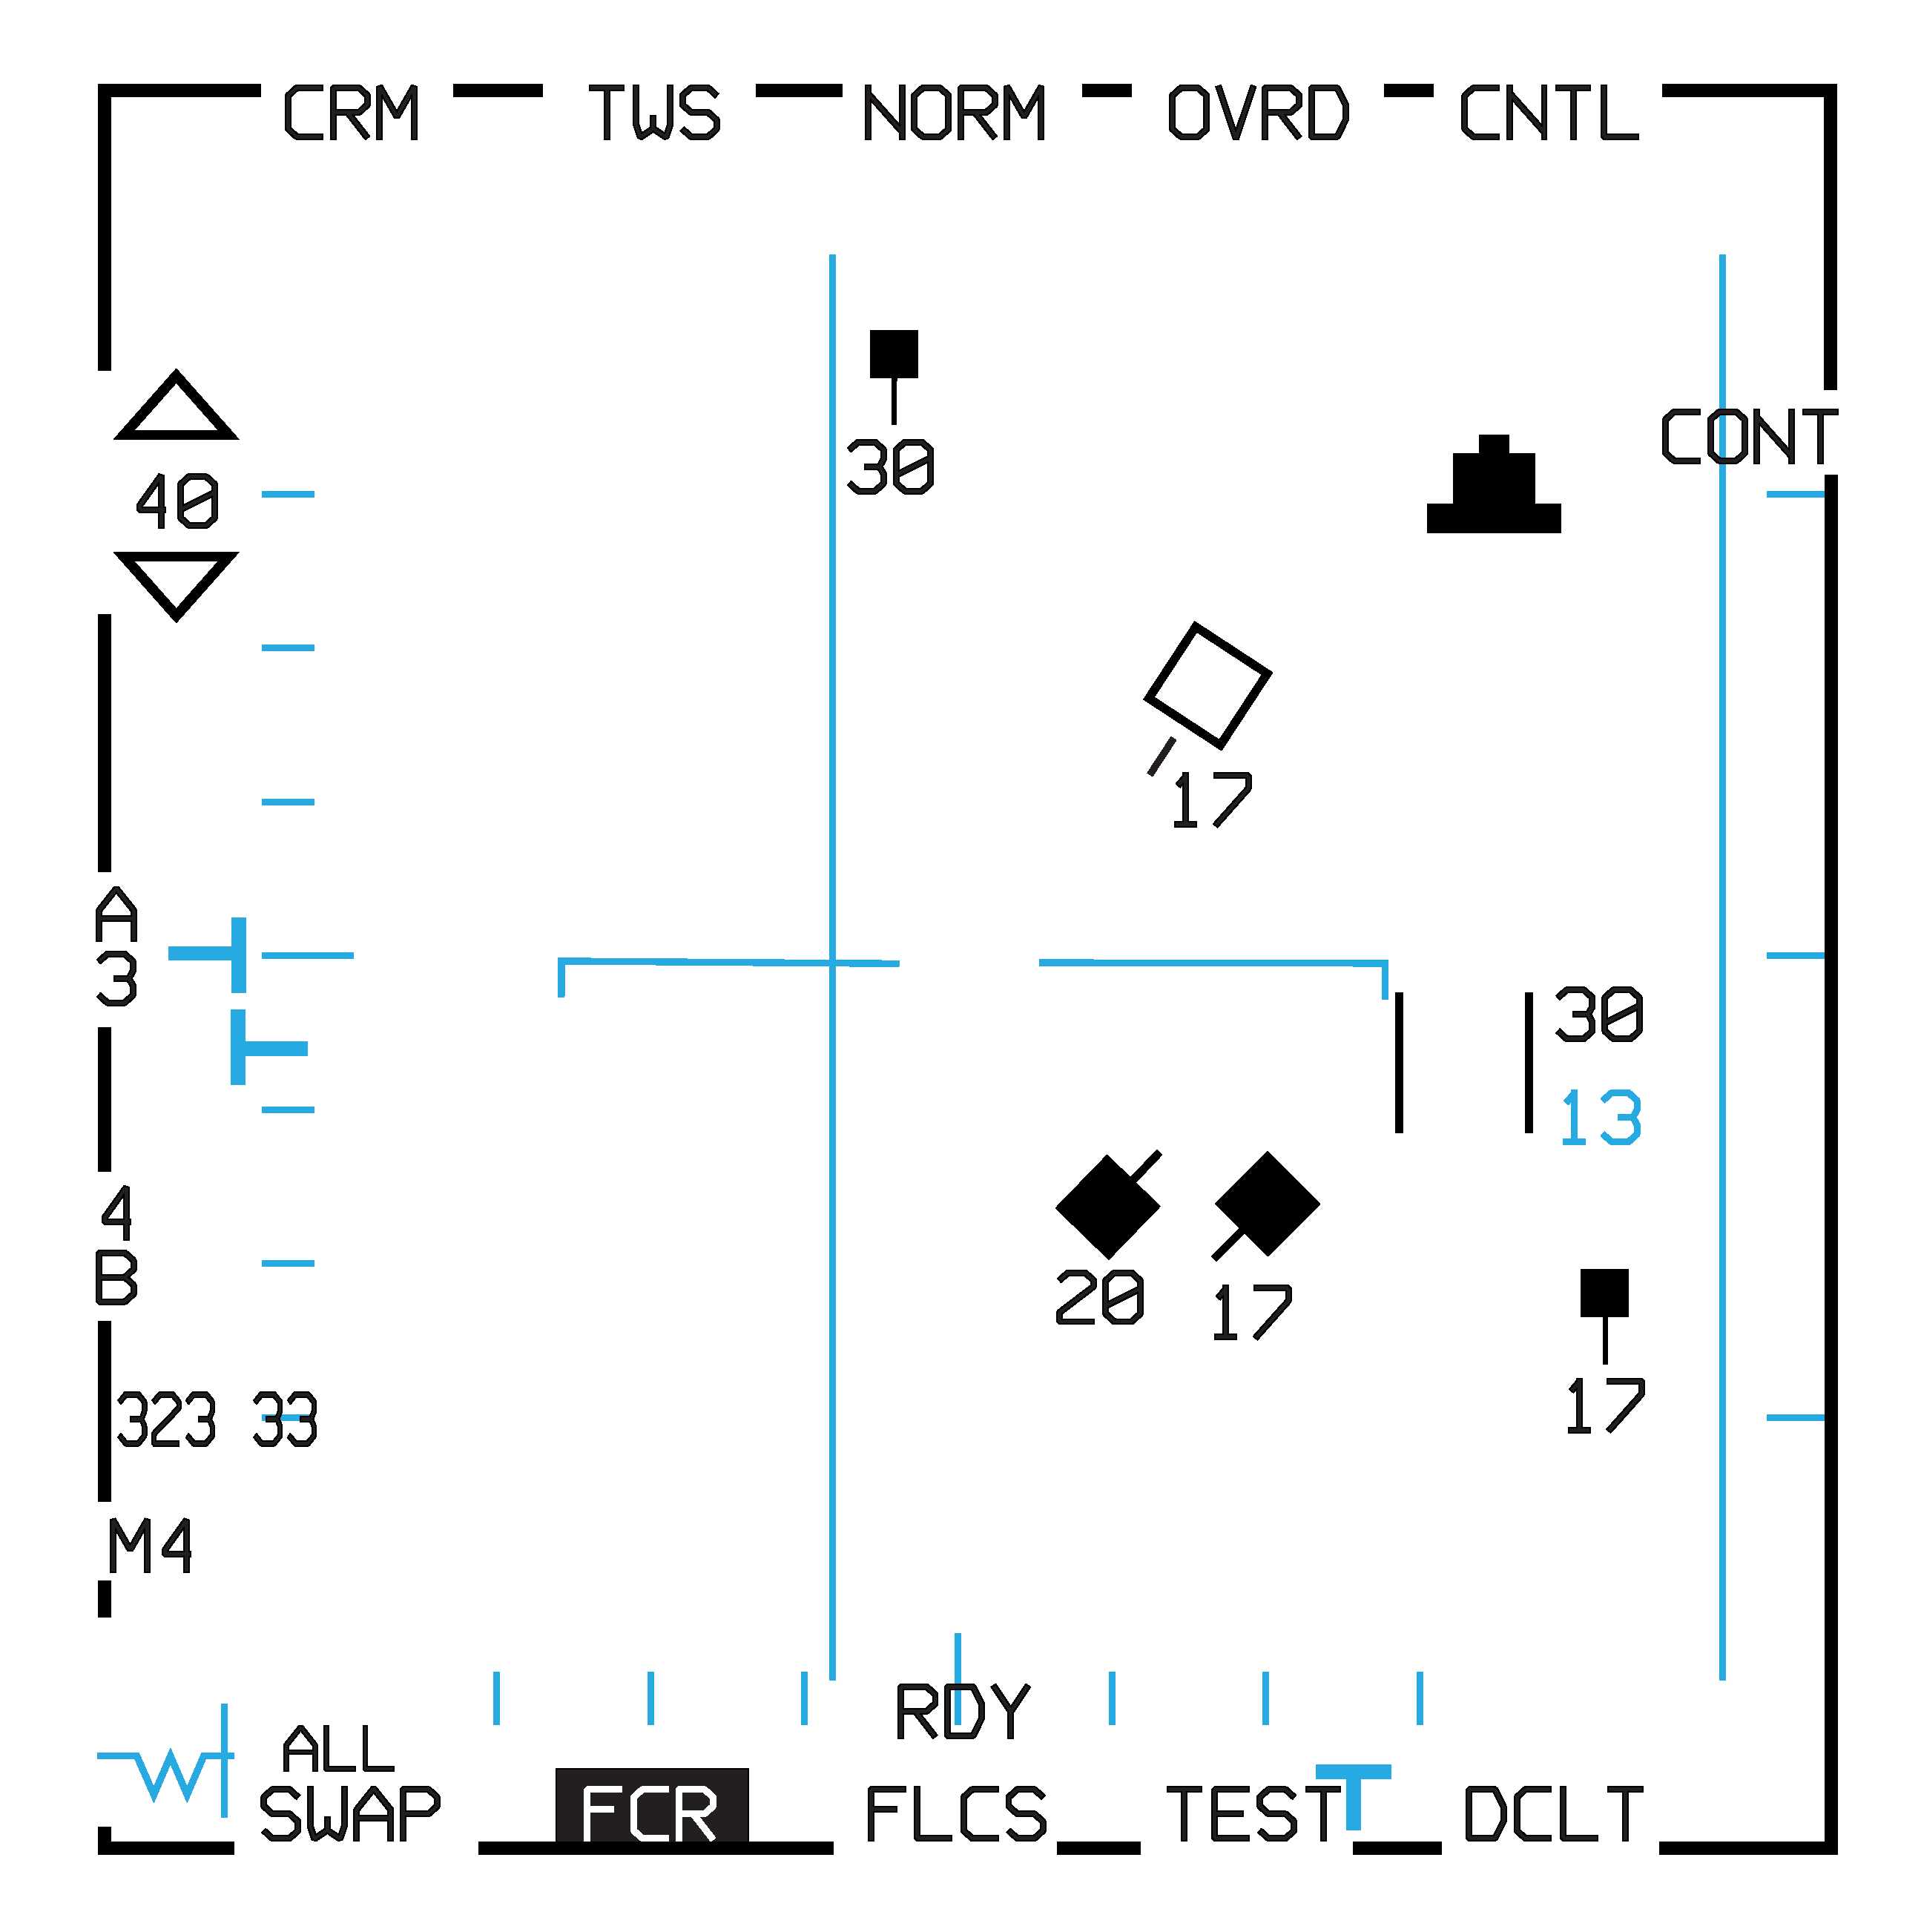
\includegraphics[
                height=75mm,
            ]{mfd/fcr_aa/tws_search.pdf}
        };

        % Annotations
        \node[lannot] (search) at ($(fig.west)+(0mm,28mm)$) {Search target};
        \draw[annotptr] (search.east) -- ++(30mm, 0mm) -- ++(4mm, -4mm);

        \node[lannot] (sec) at ($(fig.west)+(0mm,8mm)$) {Azimuth scan limits};
        \draw[annotptr] (sec.east) -- ++(32mm, 0mm);

        \node[rannot] (as) at ($(fig.east)+(0mm,24mm)$) {Current STPT};
        \draw[annotptr] (as.west) -- ++(-12mm, 0mm) -- ++(-3mm, -3mm);

        \node[rannot] (system) at ($(fig.east)+(0mm,10mm)$) {System \\ target};
        \draw[annotptr] (system.west) -- ++(-26mm, 0mm);

        \node[rannot] (cursor) at ($(fig.east)+(0mm,-4mm)$) {Acquisition cursor};
        \draw[annotptr] (cursor.west) -- ++(-11mm, 0mm);

        \node[rannot] (searchr) at ($(fig.east)+(0mm,-15mm)$) {Search \\ target};
        \draw[annotptr] (searchr.west) -- ++(-11mm, 0mm);

        \node[rannot] (asec) at ($(fig.east)+(0mm,-26mm)$) {Track \\ targets};
        \draw[annotptr] (asec.west) -- ++(-20mm, 0mm) -- ++(-6mm,10mm);
    \end{tikzpicture}
    \caption{Basic TWS search FCR page symbology.}
    \label{fig:sensors_aa:apg68:tws:search}
\end{figure}

\begin{figure}[htbp]
    \centering
    \begin{subfigure}[b]{0.15\linewidth}
        \centering
        
\includegraphics[
            scale=0.75,
        ]{mfd/fcr_aa/tgt_search.pdf}
        \caption{Search}
        \label{fig:sensorsaa:apg68:tws:trackfile:search}
    \end{subfigure}
    \begin{subfigure}[b]{0.15\linewidth}
        \centering
        
\includegraphics[
            scale=0.75,
        ]{mfd/fcr_aa/tgt_track.pdf}
        \caption{Track}
        \label{fig:sensorsaa:apg68:tws:trackfile:track}
    \end{subfigure}
    \begin{subfigure}[b]{0.15\linewidth}
        \centering
        
\includegraphics[
            scale=0.75,
        ]{mfd/fcr_aa/tgt_system.pdf}
        \caption{System}
        \label{fig:sensorsaa:apg68:tws:trackfile:system}
    \end{subfigure}
    \begin{subfigure}[b]{0.15\linewidth}
        \centering
        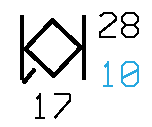
\includegraphics[
            scale=0.75,
        ]{mfd/fcr_aa/tgt_cursor.pdf}
        \caption{Cursor}
        \label{fig:sensorsaa:apg68:tws:trackfile:cursor}
    \end{subfigure}
    \begin{subfigure}[b]{0.15\linewidth}
        \centering
        
\includegraphics[
            scale=0.75,
        ]{mfd/fcr_aa/tgt_bugged.pdf}
        \caption{Bugged}
        \label{fig:sensorsaa:apg68:tws:trackfile:bugged}
    \end{subfigure}
    \caption{TWS Track Symbols}
    \label{fig:sensorsaa:apg68:tws:trackfile}
\end{figure}

\subsubsection{TRACKFILE STATES}
\label{subsec:sensorsaa:apg68:tws:trackfile}
\begin{tcoloritemize}
    \blueitem[Search Target]

    \textbf{Initial state for radar returns}
    \begin{itemize}
        \item not enough information to generate track
        \item automatic transition to track after 1-2 radar sweeps
        \item \textbf{Display} --- similar to RWS radar brick
    \end{itemize}

    Reference \cref{fig:sensorsaa:apg68:tws:trackfile:search}
    \blueitem[Track Target]
    
    \textbf{FCR automatically correlates radar return data to form track files}
    \begin{itemize}
    \item tracks target velocity, angle, altitude etc.
    \item \textbf{\underline{maximum of 10 trackfiles}}, lowest priority dropped if exceeded
    \item can be manually transitioned to higher modes by pilot to prioritize
    \end{itemize}

    Reference \cref{fig:sensorsaa:apg68:tws:trackfile:track}
    \blueitem[System Target]
    
    \textbf{Allows pilot to designate targets of interest}
    \begin{itemize}
        \item for monitoring
        \item for future weapons employment
        \item \textbf{no additional radar energy allocated to System Targets}
    \end{itemize}

    Reference \cref{fig:sensorsaa:apg68:tws:trackfile:system}
    \blueitem[Cursor Target]
        
    \textbf{Acquisition Cursor ``snaps'' to nearby System Targets} --- therefore named Cursor Targets
    \begin{itemize}
        \item \textbf{scan centered on Cursor Target}
        \begin{itemize}
            \item 3 bar elevation
            \item $\pm$25 deg azimuth pattern 
            \item reduces chance of losing track
        \end{itemize}
    \end{itemize}

    Reference \cref{fig:sensorsaa:apg68:tws:trackfile:cursor,fig:sensorsaa:apg68:tws:cursorsymb}
    \blueitem[Bugged Target]
        
    \textbf{Selected for weapons employment}
    \begin{itemize}
        \item can guide AIM-120C (w/o STT Lock)
        \item DLZ displayed if missile selected
        \item launched AIM-120 will continue to guide even if another target is bugged --- \textbf{\underline{allows for multi-target engagement}} 
        \item \textbf{scan Centered on Bugged Target}
        \begin{itemize}
            \item 3 bar elevation
            \item $\pm$25 deg azimuth pattern 
            \item reduces chance of losing track
        \end{itemize}
        \item \textbf{TMS Right --- Cycles through System Targets in range order} (bugs closest if none bugged)
    \end{itemize}

    Reference \cref{fig:sensorsaa:apg68:tws:trackfile:bugged,fig:sensorsaa:apg68:tws:buggedsymb}
    \blueitem[Spotlight] \textbf{Narrow scan centered on acquisition cursor}
    \begin{itemize}
        \item \textbf{narrow scan}
        \begin{itemize}
            \item 4 bar elevation 
            \item \pm10 deg azimuth
        \end{itemize}
        \item allows pilot to override TWS scan priority
        \item \textbf{activated by holding TMS Forward >1 sec}
    \end{itemize}
\end{tcoloritemize}

\begin{figure}[htbp]
    \centering
    \begin{tikzpicture}[auto, node distance=10mm, x=1mm, y=1mm, very thick, line cap=round,
        >={Latex[round]}
        ]
        
        \node[] (mfd) at (0,0) {
            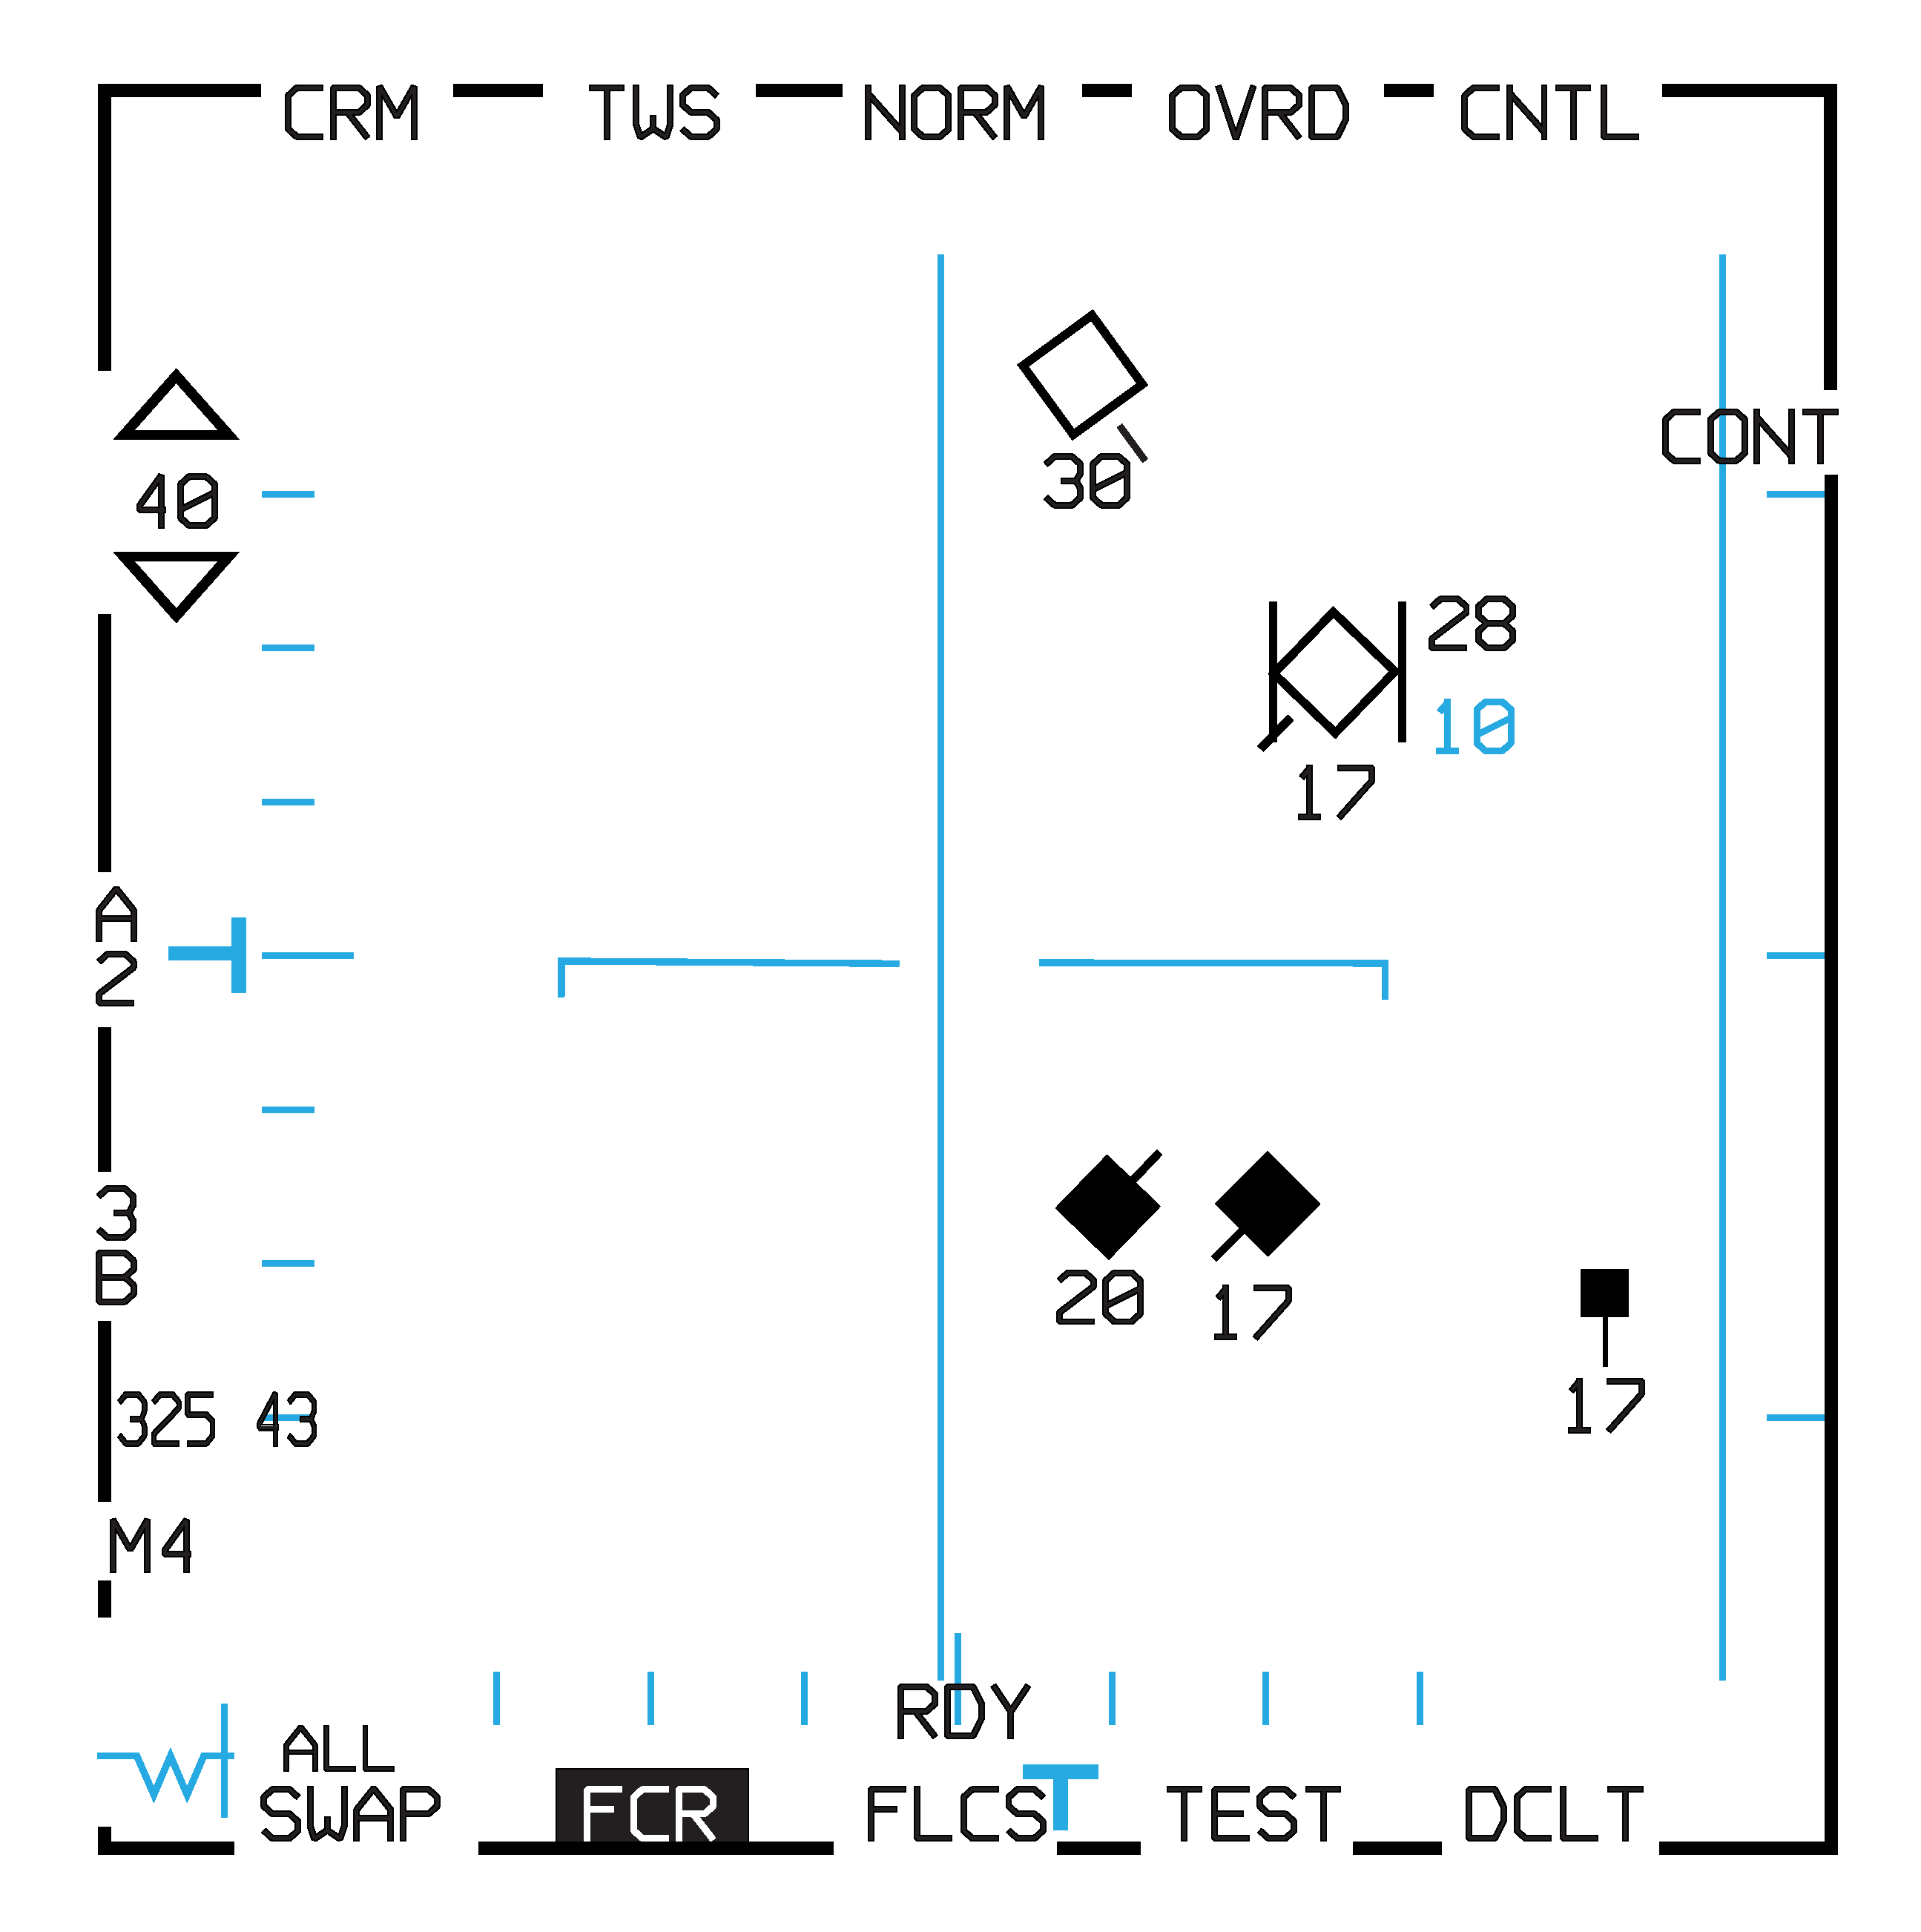
\includegraphics[
                height=75mm,
            ]{mfd/fcr_aa/tws_cursor.pdf}
        };

        % Annotations
        \node[lannot] (system) at ($(fig.west)+(0mm,29mm)$) {System \\ target};
        \draw[annotptr] (system.east) -- ++(37mm, 0mm) -- ++(4mm, -4mm);

        \node[lannot] (sec) at ($(fig.west)+(0mm,8mm)$) {Azimuth scan limits};
        \draw[annotptr] (sec.east) -- ++(36mm, 0mm);

        \node[rannot] (cursor) at ($(fig.east)+(0mm,11mm)$) {Cursor \\ target};
        \draw[annotptr] (cursor.west) -- ++(-15mm, 0mm);

        \node[rannot] (searchr) at ($(fig.east)+(0mm,-15mm)$) {Search \\ target};
        \draw[annotptr] (searchr.west) -- ++(-11mm, 0mm);

        \node[rannot] (asec) at ($(fig.east)+(0mm,-26mm)$) {Track \\ targets};
        \draw[annotptr] (asec.west) -- ++(-20mm, 0mm) -- ++(-6mm,10mm);
    \end{tikzpicture}
    \caption{TWS FCR page symbology with cursor target}
    \label{fig:sensorsaa:apg68:tws:cursorsymb}
\end{figure}

\begin{figure}[htbp]
    \centering
    \begin{tikzpicture}[auto, node distance=10mm, x=1mm, y=1mm, very thick, line cap=round,
        >={Latex[round]}
        ]
        
        \node[] (mfd) at (0,0) {
            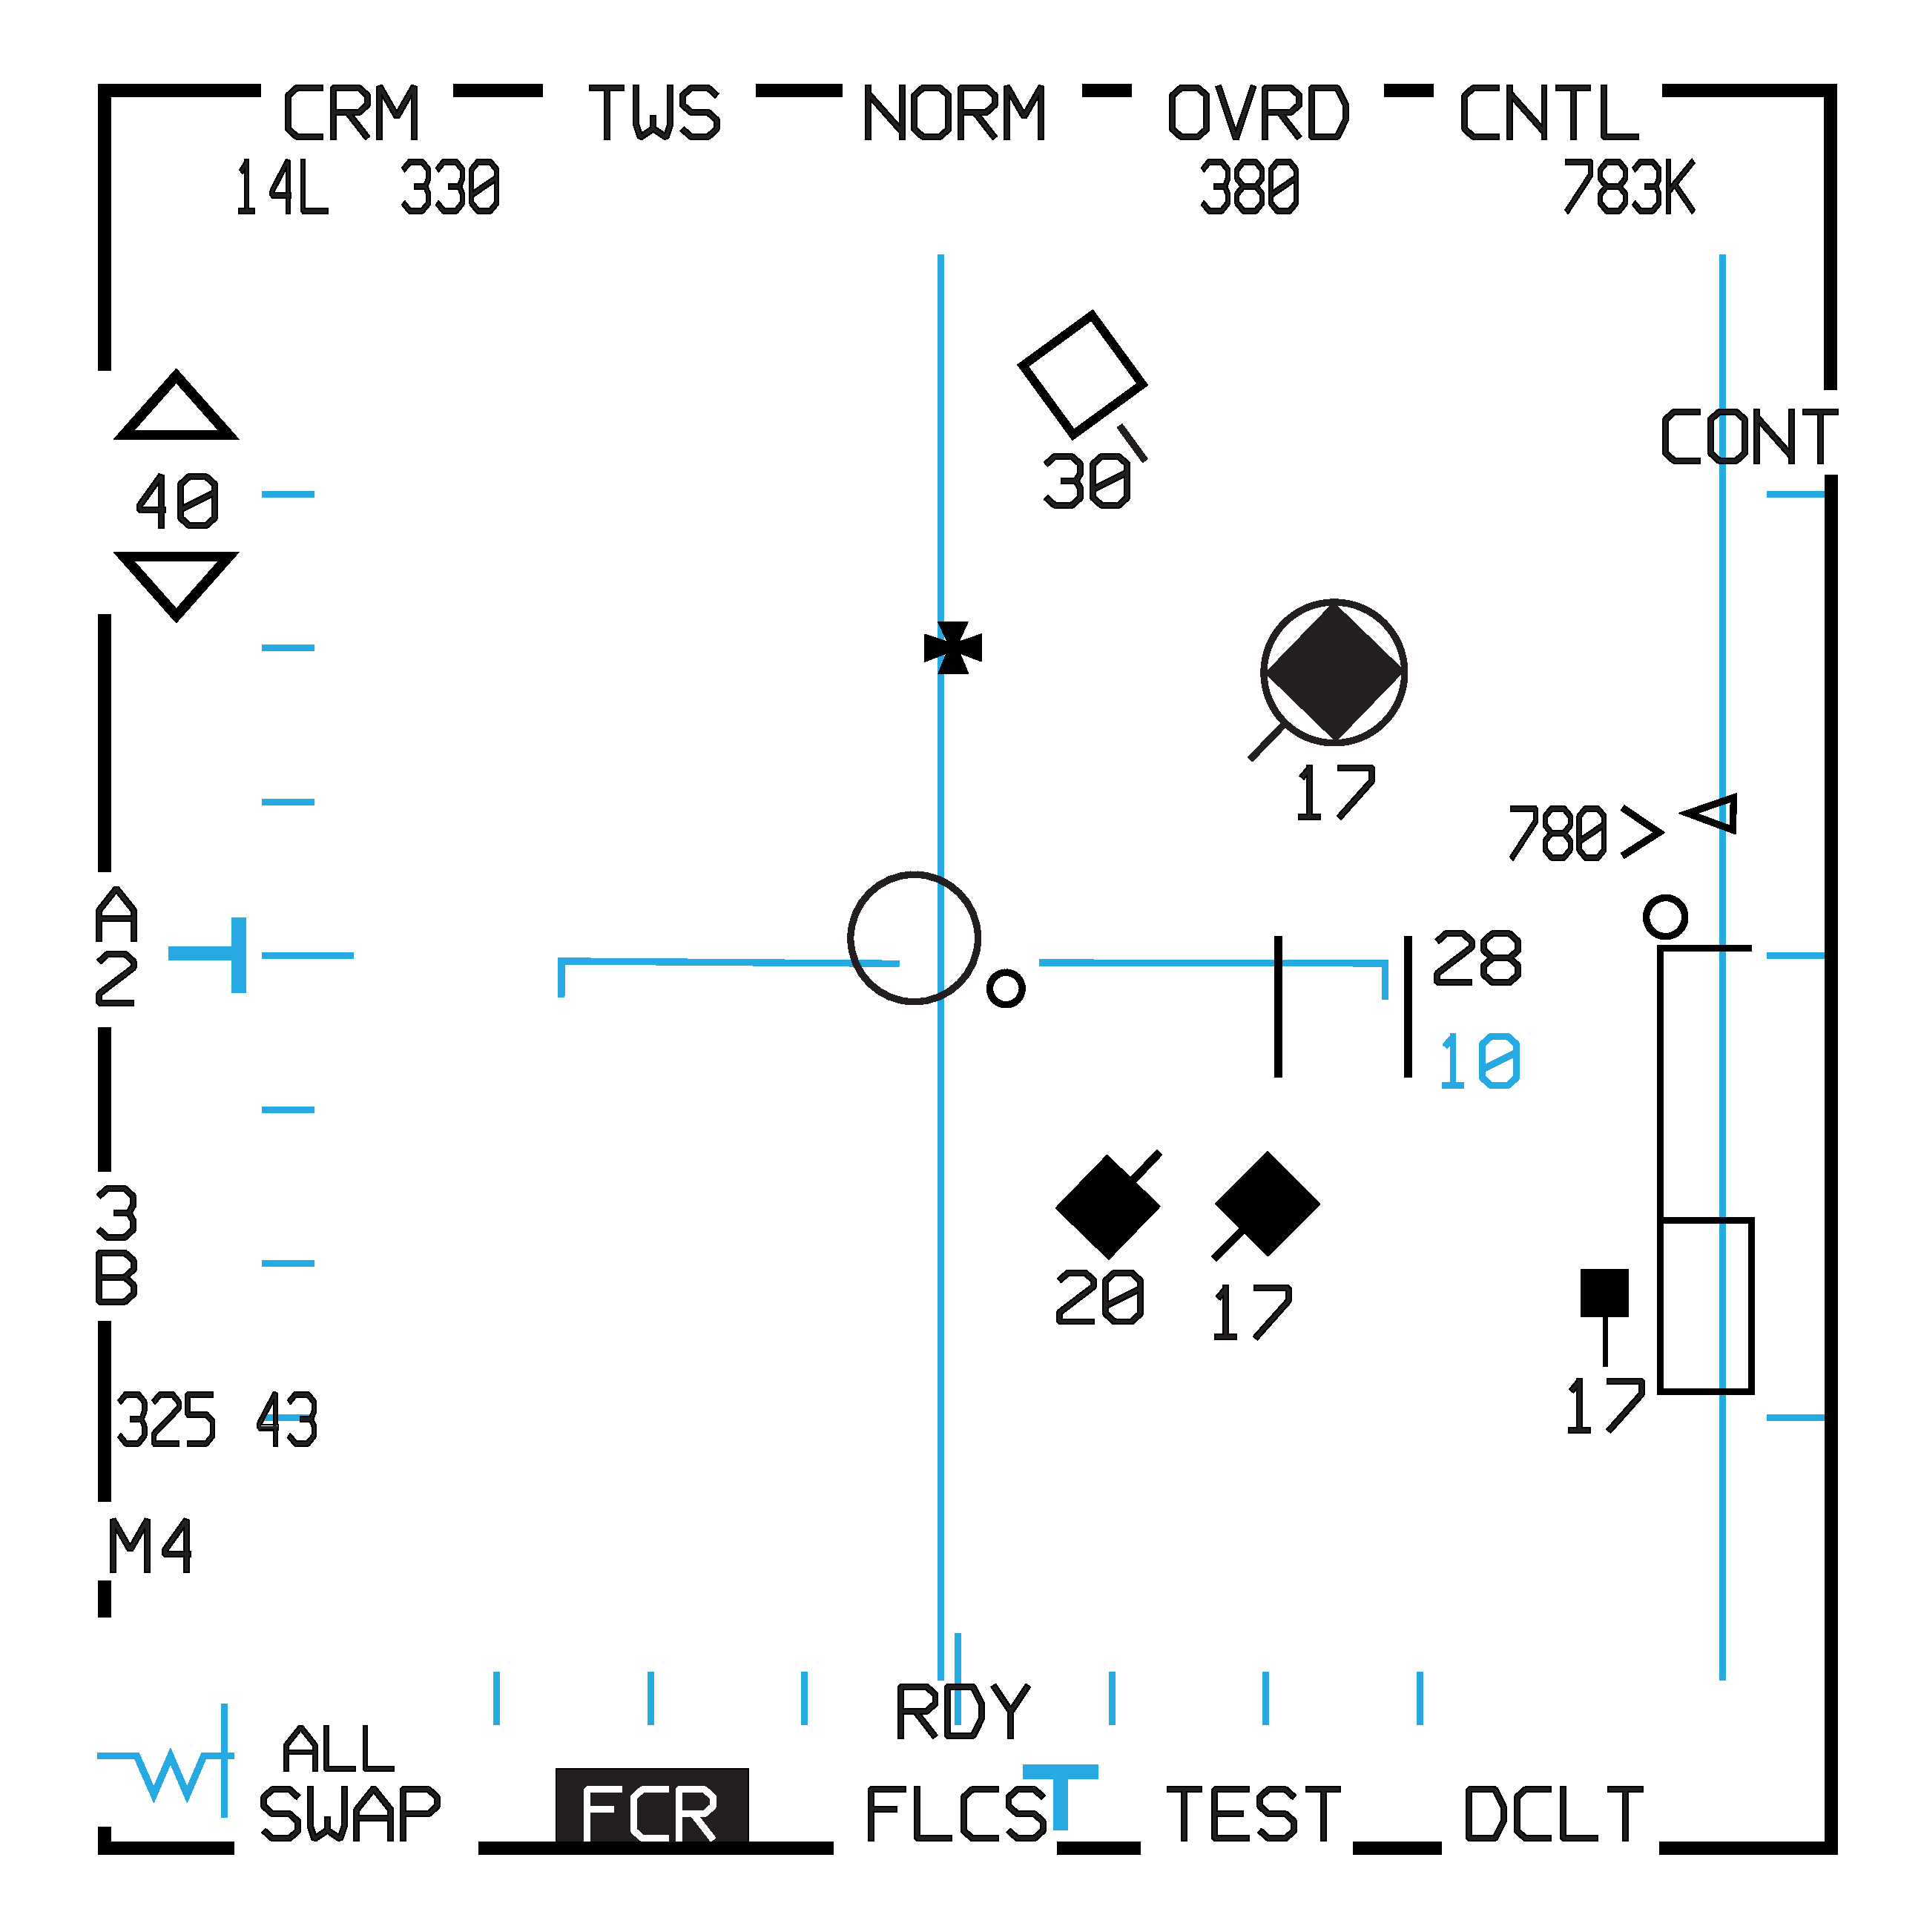
\includegraphics[
                height=75mm,
            ]{mfd/fcr_aa/tws_bugged.pdf}
        };

        % Annotations
        \node[lannot] (asp) at ($(fig.west)+(0mm,30.25mm)$) {Aspect};
        \draw[annotptr] (asp.east) -- ++(9mm, 0mm);

        \node[lannot] (trk) at ($(fig.west)+(0mm,24mm)$) {Track};
        \draw[annotptr] (trk.east) -- ++(12mm, 0mm) -- ++(4mm, 4mm);

        % \node[lannot] (system) at ($(fig.west)+(0mm,15mm)$) {System \\ target};
        % \draw[annotptr] (system.east) -- ++(37mm, 0mm) -- ++(4mm, 4mm);

        \node[lannot] (cross) at ($(fig.west)+(0mm,7mm)$) {Steering \\ cross};
        \draw[annotptr] (cross.east) -- ++(32mm, 0mm) -- ++(4mm, 4mm);

        % \node[lannot] (sec) at ($(fig.west)+(0mm,-8mm)$) {Azimuth scan limits};
        % \draw[annotptr] (sec.east) -- ++(36mm, 0mm);

        \node[lannot] (asec) at ($(fig.west)+(0mm,-6mm)$) {ASC / ASEC \\ {\footnotesize see \cref{fig:aa_weap:aim120:asc_asec}}};
        \draw[annotptr] (asec.east) -- ++(30mm, 0mm) -- ++(4mm, 4mm);

        \node[rannot] (clos) at ($(fig.east)+(0mm,30.25mm)$) {Closure};
        \draw[annotptr] (clos.west) -- ++(-9mm, 0mm);

        \node[rannot] (as) at ($(fig.east)+(0mm,24mm)$) {Airspeed};
        \draw[annotptr] (as.west) -- ++(-22mm, 0mm) -- ++(-4mm, 4mm);

        \node[rannot] (bug) at ($(fig.east)+(0mm,11mm)$) {Bugged \\ target};
        \draw[annotptr] (bug.west) -- ++(-20mm, 0mm);

        \node[rannot] (dlz) at ($(fig.east)+(0mm,-10mm)$) {DLZ \\ {\footnotesize see \cref{fig:aa_weap:aim120:dlz}}};
        \draw[annotptr] (dlz.west) -- ++(-7mm, 0mm);

        \node[rannot] (asec) at ($(fig.east)+(0mm,-26mm)$) {Track \\ targets};
        \draw[annotptr] (asec.west) -- ++(-20mm, 0mm) -- ++(-6mm,10mm);
    \end{tikzpicture}
    \caption{
        TWS FCR page symbology with bugged target. 
        Note that ``shoot'' symbology (DLZ, ASEC, steering cross) 
        as well as additional information about the bugged target is displayed.
    }
    \label{fig:sensorsaa:apg68:tws:buggedsymb}
\end{figure}

\marginfigeometry

\subsubsection{SELECT TWS MODE}
\begin{checklistenumerate}
    \blueitem[FCR Switch] \textbf{FCR}
    \blueitem[Desired MFD] \textbf{FCR Page}, verify \textbf{SOI}
    \blueitem[Radar Mode]
    \textbf{CRM} (default), verify

    \begin{itemize}
        \item \textbf{Dogfight/Missile Override} --- \textbf{NORM}
        \item \textbf{Radar Mode (OSB 1)} --- shows \textbf{CRM}
    \end{itemize}
    \blueitem[CRM Submode]
    \textbf{TWS}, cycle via 

    \begin{itemize}
        \item \textbf{TMS Right (long)} / \textbf{OSB 2} 
    \end{itemize}
\end{checklistenumerate}

\subsubsection{MULTI-TARGET ACQUISITION}
\label{subsec:tws:multiacq}
\begin{checklistenumerate}
    \blueitem[Track Target Acquisition]
    \label{subsec:sensorsaa:apg68:tws:multi:trk}
    \marginpar{
        \captionsetup{type=figure}
        \centering
        \begin{tikzpicture}[figstyle]
            
            \node[
                boxedmarfigstyle,            
            ] (search) at (0,0) {
                
\includegraphics[
                    scale=0.5,
                ]{mfd/fcr_aa/tgt_search.pdf}
            };
            \node[
                boxedmarfigstyle,               
                below=10 of search,
            ] (track) {
                
\includegraphics[
                    scale=0.5,
                ]{mfd/fcr_aa/tgt_track.pdf}
            };
            \node[
                boxedmarfigstyle,
                below=17.5 of track,
            ] (system) {
                
\includegraphics[
                    scale=0.5,
                ]{mfd/fcr_aa/tgt_system.pdf}
            };
            \node[
                boxedmarfigstyle,                
                below=12.5 of system,
            ] (cursor) {
                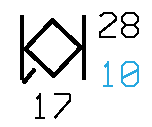
\includegraphics[
                    scale=0.5,
                ]{mfd/fcr_aa/tgt_cursor.pdf}
            };
            \node[
                boxedmarfigstyle,                
                below=10 of cursor,
            ] (bugged) {
                
\includegraphics[
                    scale=0.5,
                ]{mfd/fcr_aa/tgt_bugged.pdf}
            };

            % lines
            \draw[->]
            (search) -- node[right, align=left, font=\small] {\textbf{Automatic}}(track);
            \path (search) -- node[left, align=right, font=\small] {\ref{subsec:sensorsaa:apg68:tws:multi:trk}}(track);
            \draw[->]
            (track) -- node[right, align=left, font=\small] {\textbf{TMS FWD} \\ \footnotesize\textbf{(repeat for all} \\ \footnotesize\textbf{desired targets)}}(system);
            \draw[>-]
            ($(track.south)!0.5!(system.north) + (-5,0)$) -- ++(0,2) arc (180:0:2.5) -- ++(0,-4) arc (360:180:2.5) -- node[left, align=right, font=\small, pos=1] {\ref{subsec:sensorsaa:apg68:tws:multi:sys}} ++(0,2);
            \draw[->]
            (system) -- node[right, align=left, font=\small] {\textbf{Slew Cursor} \\ \textbf{near target}}(cursor);
            \draw[->]
            (cursor) -- node[right, align=left, font=\small] {\textbf{TMS FWD}}(bugged);
            \path (cursor) -- node[left, align=right, font=\small] {\ref{subsec:sensorsaa:apg68:tws:multi:bug}}(bugged);

            % labels
            \node[
                anchor=north west,
                align=left,
                font=\bfseries\footnotesize,
            ] (labelsearch) at (search.north west) {Search \\ Target};
            \node[
                anchor=north west,
                align=left,
                font=\bfseries\footnotesize,
            ] (labeltrack) at (track.north west) {Track \\ Target};
            \node[
                anchor=north west,
                align=left,
                font=\bfseries\footnotesize,
            ] (labelsystem) at (system.north west) {System \\ Target};
            \node[
                anchor=north west,
                align=left,
                font=\bfseries\footnotesize,
            ] (labelcursor) at (cursor.north west) {Cursor \\ Target};
            \node[
                anchor=north west,
                align=left,
                font=\bfseries\footnotesize,
            ] (labelbugged) at (bugged.north west) {Bugged \\ Target};
        \end{tikzpicture}
        \caption{TWS trackfile acquisition flow}
    }
    \begin{enumerate}
        \item Correlate onboard/offboard sensors to locate targets
        \begin{itemize}
            \item raw radar returns, RWR pings
            \item AWACS calls, datalink targets
        \end{itemize}
        \item Place targets within radar scan volume
        \item FCR automatically generates Track Targets once sufficient data available
    \end{enumerate}
    \blueitem[System Target Acquisition]
    \label{subsec:sensorsaa:apg68:tws:multi:sys}
    \begin{enumerate}
        \item \textbf{Target} \dotfill under Acquisition Cursor
        \item \textbf{TMS} \dotfill \textbf{Forward} 
    \end{enumerate}
    Repeat for all desired Track Targets,
    or to upgrade all Track Targets:
    \begin{enumerate}
        \item \textbf{TMS} \dotfill \textbf{Right}
    \end{enumerate}
    \blueitem[Upgrade to Bugged Target]
    \label{subsec:sensorsaa:apg68:tws:multi:bug}
    \begin{enumerate}
        \item \textbf{Target} \dotfill under Acquisition Cursor
        \item \textbf{TMS} \dotfill \textbf{Forward}
    \end{enumerate}
    To select closest System Target 
    \begin{enumerate}
        \item \textbf{TMS} \dotfill \textbf{Right}
    \end{enumerate}
    To cycle through System Targets in range order
    \begin{enumerate}
        \item \textbf{TMS} \dotfill \textbf{Right}
    \end{enumerate}
    \blueitem[STT Lock] (if desired)
    \begin{enumerate}
        \item \textbf{Bugged Target} \dotfill under Acq Cursor
        \item \textbf{TMS} \dotfill \textbf{Forward}
    \end{enumerate}
\end{checklistenumerate}

\marginfigrestore

\subsection{ACM}
\label{subsec:acm}
\begin{tcoloritemize}
    \blueitem{ACM}{
    \textbf{A}ir \textbf{C}ombat \textbf{M}ode

    \begin{subitemize}
        \item \textbf{Used to automatically lock targets while maneuvering}
        \item \textbf{Sub-Modes}
        \begin{itemize}
            \item \textbf{HUD Scan} --- 30x20 deg 
            \item \textbf{BORE} --- Boresight (3x3 deg)
            \item \textbf{Vertical Scan} --- 10x60 deg
            \item \textbf{Slewable} --- WIP
        \end{itemize}
    \end{subitemize}}
\end{tcoloritemize}

\begin{figure}[htbp]
    \centering
    \begin{tikzpicture}[auto, node distance=10mm, x=1mm, y=1mm, very thick,
        >={Latex[round]}
        ]
        
        % \node[<options>](<coordinate name>)at(<coordinate>){<text>};
        \node[
            hyperref node=subsec:acm,
            rectangle,
            rounded corners,
            minimum width=15mm,
            minimum height=15mm,
            draw,
        ](acm)at(0,0){\blue{ACM}};
        \node[
            rectangle,
            rounded corners,
            minimum width=20mm,
            minimum height=7.5mm,
            draw,
        ](bore)at(0,20){\textbf{BORE}};
        \node[
            rectangle,
            rounded corners,
            minimum width=20mm,
            minimum height=7.5mm,
            draw,
        ](hud)at(32.5,0){\textbf{HUD}};
        \node[
            rectangle,
            rounded corners,
            minimum width=20mm,
            minimum height=7.5mm,
            draw,
        ](vert)at(0,-20){\textbf{Vertical}};
        \node[
            hyperref node=subsec:stt,
            rectangle, 
            rounded corners,
            minimum width=90mm,
            minimum height=7.5mm,
            draw, 
        ](stt)at(0,35){\blue{STT}};
                
        % Lines
        \draw [->]
            (acm) -- node[pos=0.5, left]{\scriptsize\textbf{TMS FWD}} (bore);
        \draw [->]
            (acm) -- node[pos=0.5, above]{\scriptsize\textbf{TMS}}node[pos=0.5, below]{\scriptsize\textbf{RIGHT}} (hud);
        \draw [->]
            (acm) -- node[pos=0.5, left]{\scriptsize\textbf{TMS AFT}} (vert);
        \draw [->]
            let
                \p1=(bore.north),
                \p2=(stt.south),
            in
                (\p1) -- node[pos=0.5, left]{\scriptsize\textbf{Automatic}} (\x1,\y2);
        \draw [->]
            let
                \p1=(hud.north),
                \p2=(stt.south),
            in
                (\p1) -- node[pos=0.5, left]{\scriptsize\textbf{Automatic}} (\x1,\y2);
        \draw [->, rounded corners]
            let
                \p1=(vert.west),
                \p2=(stt.south),
            in
                (\p1) -- (\x1-22.5mm,\y1) -- node[pos=0.5, left]{\scriptsize\textbf{Automatic}} (\x1-22.5mm,\y2);
                
    \end{tikzpicture}
    \caption{ACM Radar Modes Overview}
    \label{fig:acmoverview}
\end{figure}

\begin{figure}[htbp]
    \centering
    \begin{tikzpicture}[auto, node distance=10mm, x=1mm, y=1mm, very thick, line cap=round,
        >={Latex[round]}
        ]
        
        \node[] (fig) at (0,0) {
            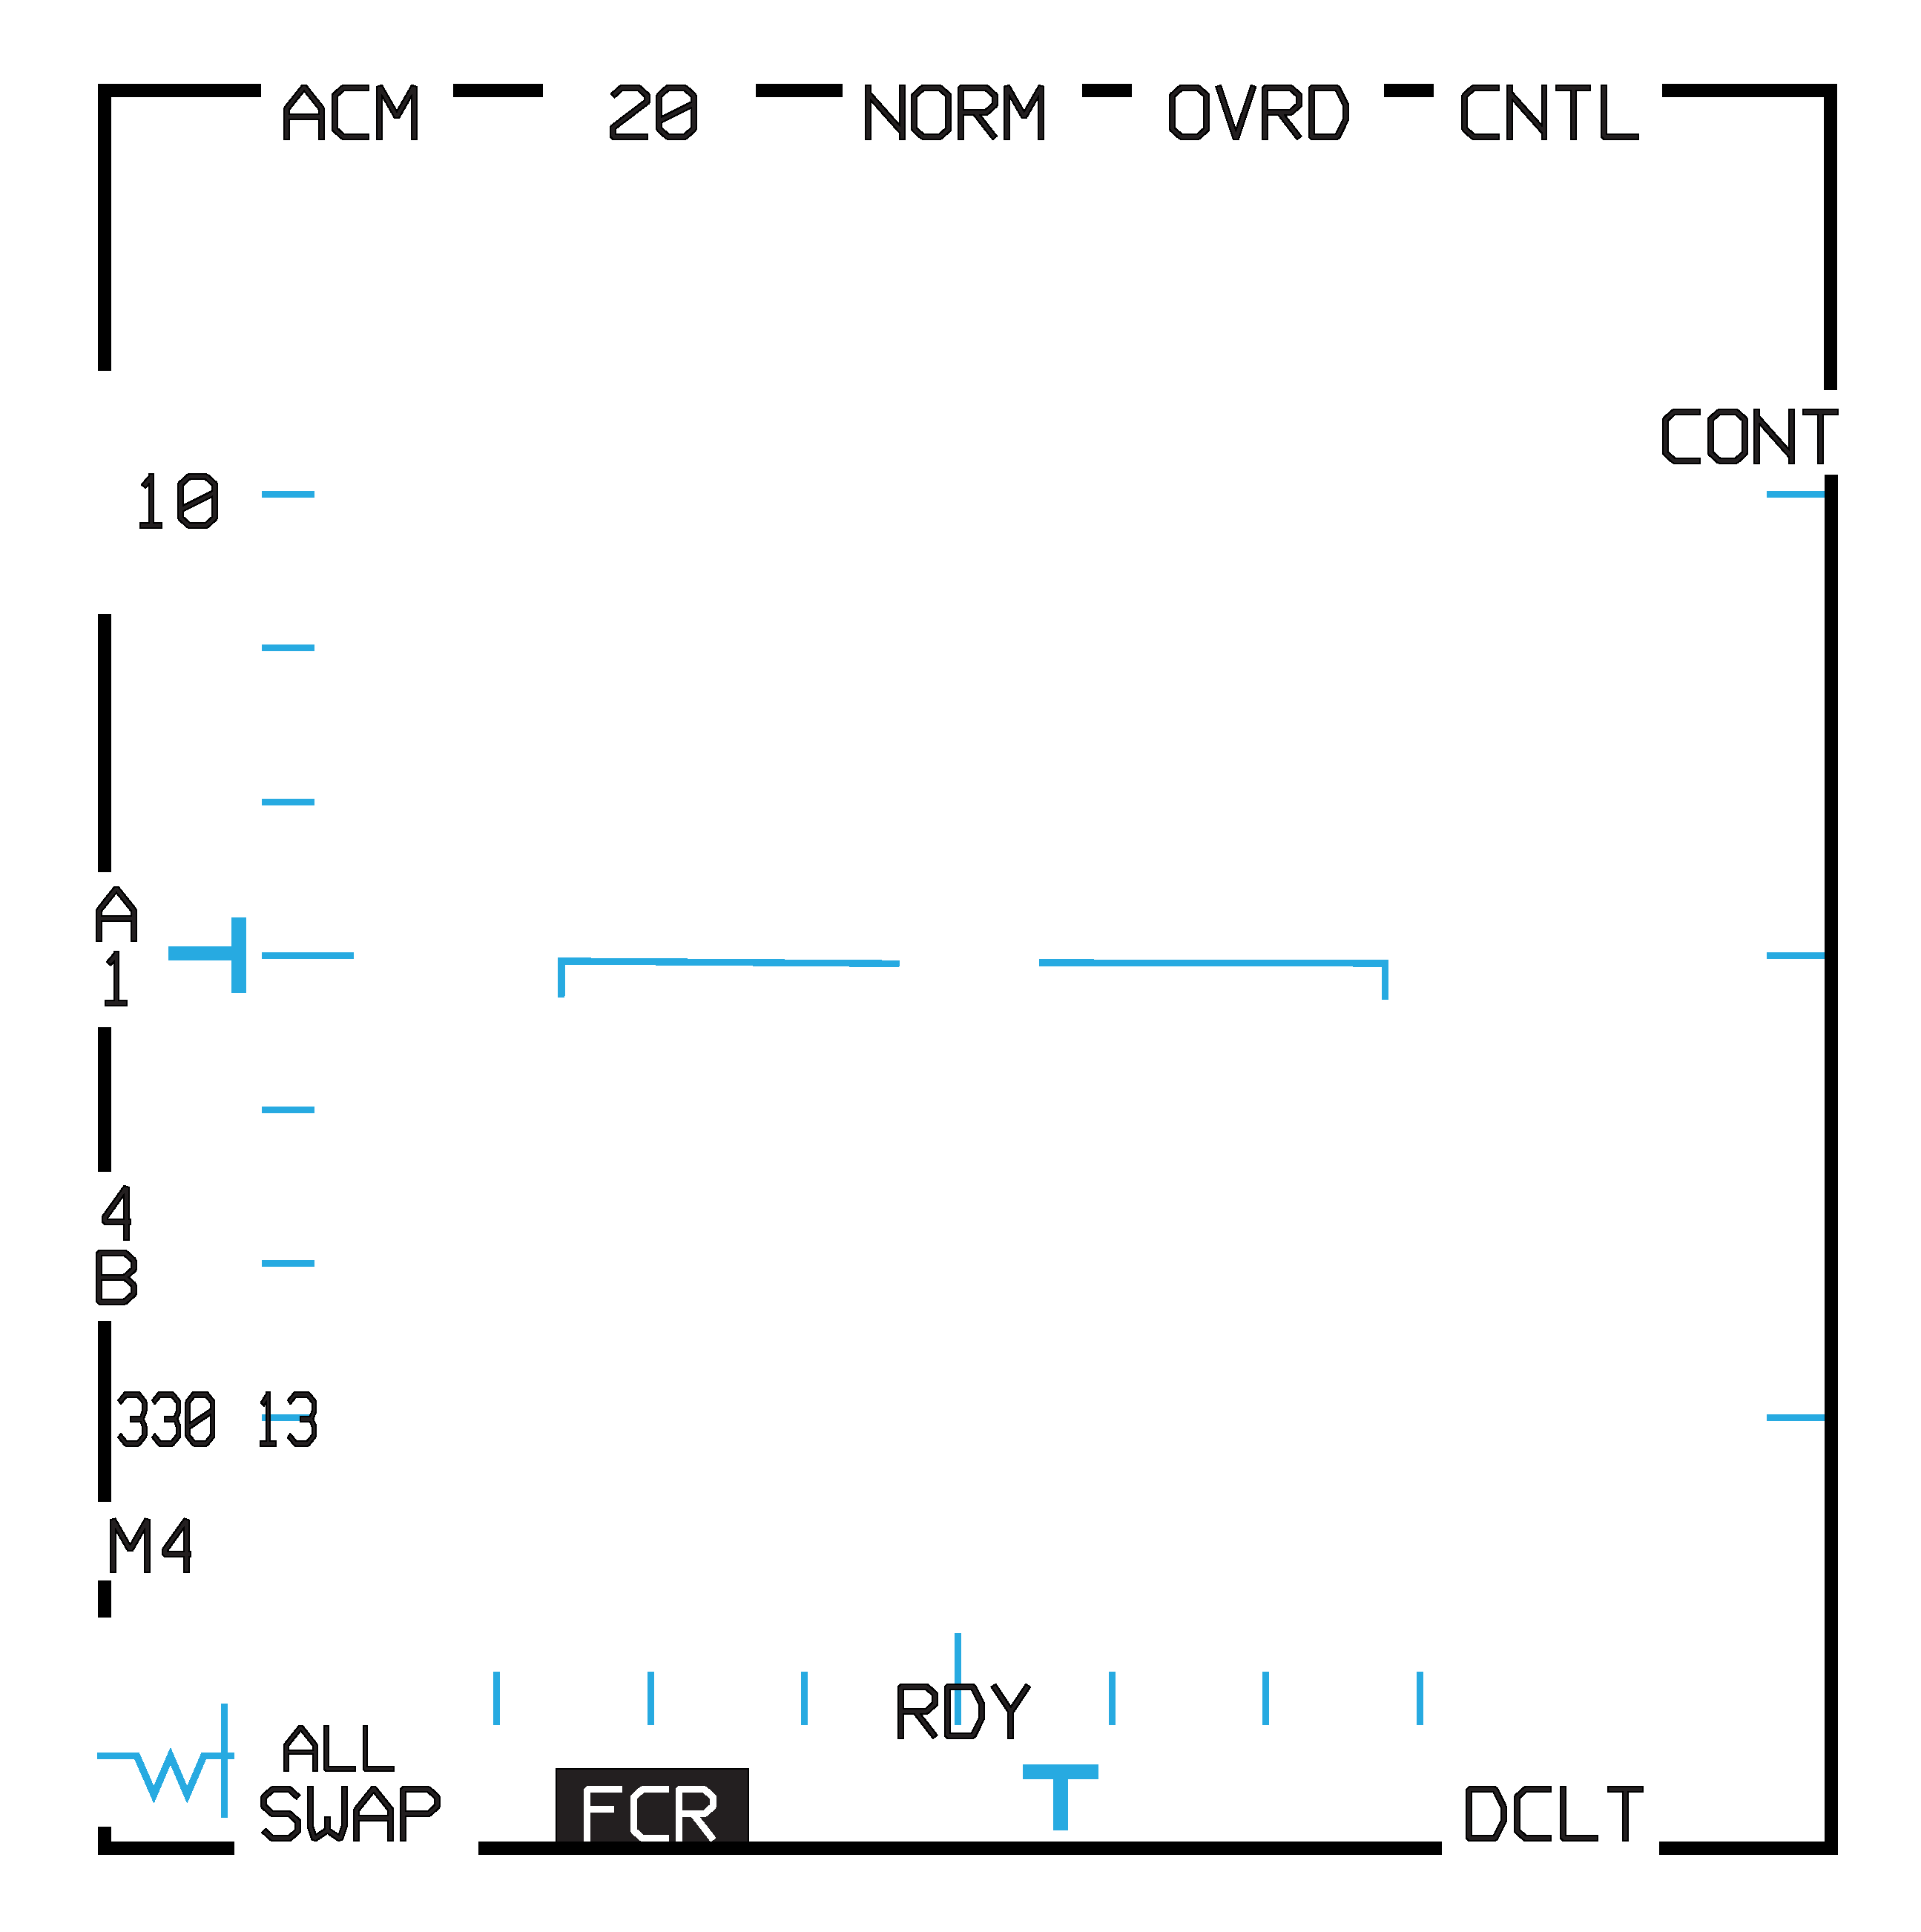
\includegraphics[
                height=75mm,
            ]{mfd/fcr_aa/acm_homepage.pdf}
        };

        % Annotations
        \node[lannot] (mode) at ($(fig.west)+(0mm,38mm)$) {FCR mode};
        \draw[->, red] (mode.east) -- ++(12mm, 0mm) -- (-24mm,35mm);

        \node[lannot] (submode) at ($(fig.west)+(0mm,28mm)$) {ACM \\ submode};
        \draw[->, red] (submode.east) -- ++(23mm, 0mm) -- (-13mm, 31mm);

        \node[lannot] (rsel) at ($(fig.west)+(0mm,18mm)$) {Range scale};
        \draw[->, red] (rsel.east) -- ++(4.5mm, 0mm);

        \node[lannot] (asel) at ($(fig.west)+(0mm,0.5mm)$) {Azimuth};
        \draw[->, red] (asel.east) -- ++(4.5mm, 0mm);

        \node[lannot] (bsel) at ($(fig.west)+(0mm,-10.5mm)$) {Elevation \\ bar};
        \draw[->, red] (bsel.east) -- ++(4.5mm, 0mm);

        \node[annot, anchor=south, align=center] (fov) at ($(fig.north)+(0mm,0mm)$) {FOV select};
        \draw[->, red] (fov.south) -- ++(0mm, -3.5mm);

        \node[rannot] (cntl) at ($(fig.east)+(0mm,38mm)$) {Control};
        \draw[->, red] (cntl.west) -- ++(-13mm, 0mm) -- (23mm, 35mm);

        \node[rannot] (ovrd) at ($(fig.east)+(0mm,28mm)$) {Override};
        \draw[->, red] (ovrd.west) -- ++(-24mm, 0mm) -- (12mm, 31mm);

        \node[rannot] (dl) at ($(fig.east)+(0mm,20.5mm)$) {Datalink mode};
        \draw[->, red] (dl.west) -- ++(-4mm,0mm);

        \node[rannot] (sj) at ($(fig.east)+(0mm,-8mm)$) {Horizon \\indicator};
        \draw[->, red] (sj.west) -- ++(-20mm, 0mm) -- (12mm,-1mm);

        \node[rannot] (dclt) at ($(fig.east)+(0mm,-38mm)$) {Declutter};
        \draw[->, red] (dclt.west) -- ++(-13mm, 0mm) -- (23mm, -35mm);
    \end{tikzpicture}
    \caption{ACM FCR page symbology}
\end{figure}

\begin{figure}[htbp]
    \centering
    \begin{subfigure}[t]{0.3\linewidth}
        \centering
        \begin{tikzpicture}[figstyle]
            
            \draw[color2, fill=color2!20, dashed, rounded corners]
            (-15, 10) -- (15,10) -- (15,-10) -- (-15,-10) -- cycle;

            \node[] (fig) at (0,0) {
                
\includegraphics[
                    scale=0.25,
                ]{hud/acm/subfig_hud.pdf}
            };

        \end{tikzpicture}
        \caption{HUD}
    \end{subfigure}
    \begin{subfigure}[t]{0.3\linewidth}
        \centering
        \begin{tikzpicture}[figstyle]

            \draw[color2, fill=color2!20, dashed] 
            (0,-3) circle [x radius=4, y radius=6];
            
            \node[] (bore) at (0,0) {
                
\includegraphics[
                    scale=0.25,
                ]{hud/acm/subfig_bore.pdf}
            };
    
        \end{tikzpicture}
        \caption{BORE}
    \end{subfigure}
    \begin{subfigure}[t]{0.3\linewidth}
        \centering
        \begin{tikzpicture}[figstyle]

            \draw[color2, fill=color2!20, dashed, rounded corners]
            (-2.5, 30) -- (2.5,30) -- (2.5,-8) -- (-2.5,-8) -- cycle;
            
            \node[] (vert) at (0,0) {
                
\includegraphics[
                    scale=0.25,
                ]{hud/acm/subfig_vert.pdf}
            };
    
        \end{tikzpicture}
        \caption{Vertical}
    \end{subfigure}
    \caption{
        ACM Scan Patterns shown with the relevant HUD symbology. 
        The dashed lines indicate the scan volume for illustrative purposes and are not to scale.
    }
\end{figure}

\begin{figure}[htbp]
    \centering
    \begin{tikzpicture}[auto, node distance=10mm, x=1mm, y=1mm, very thick, line cap=round,
        >={Latex[round]}
        ]

        \node[draw, rounded corners] (fig) at (0,0) {
            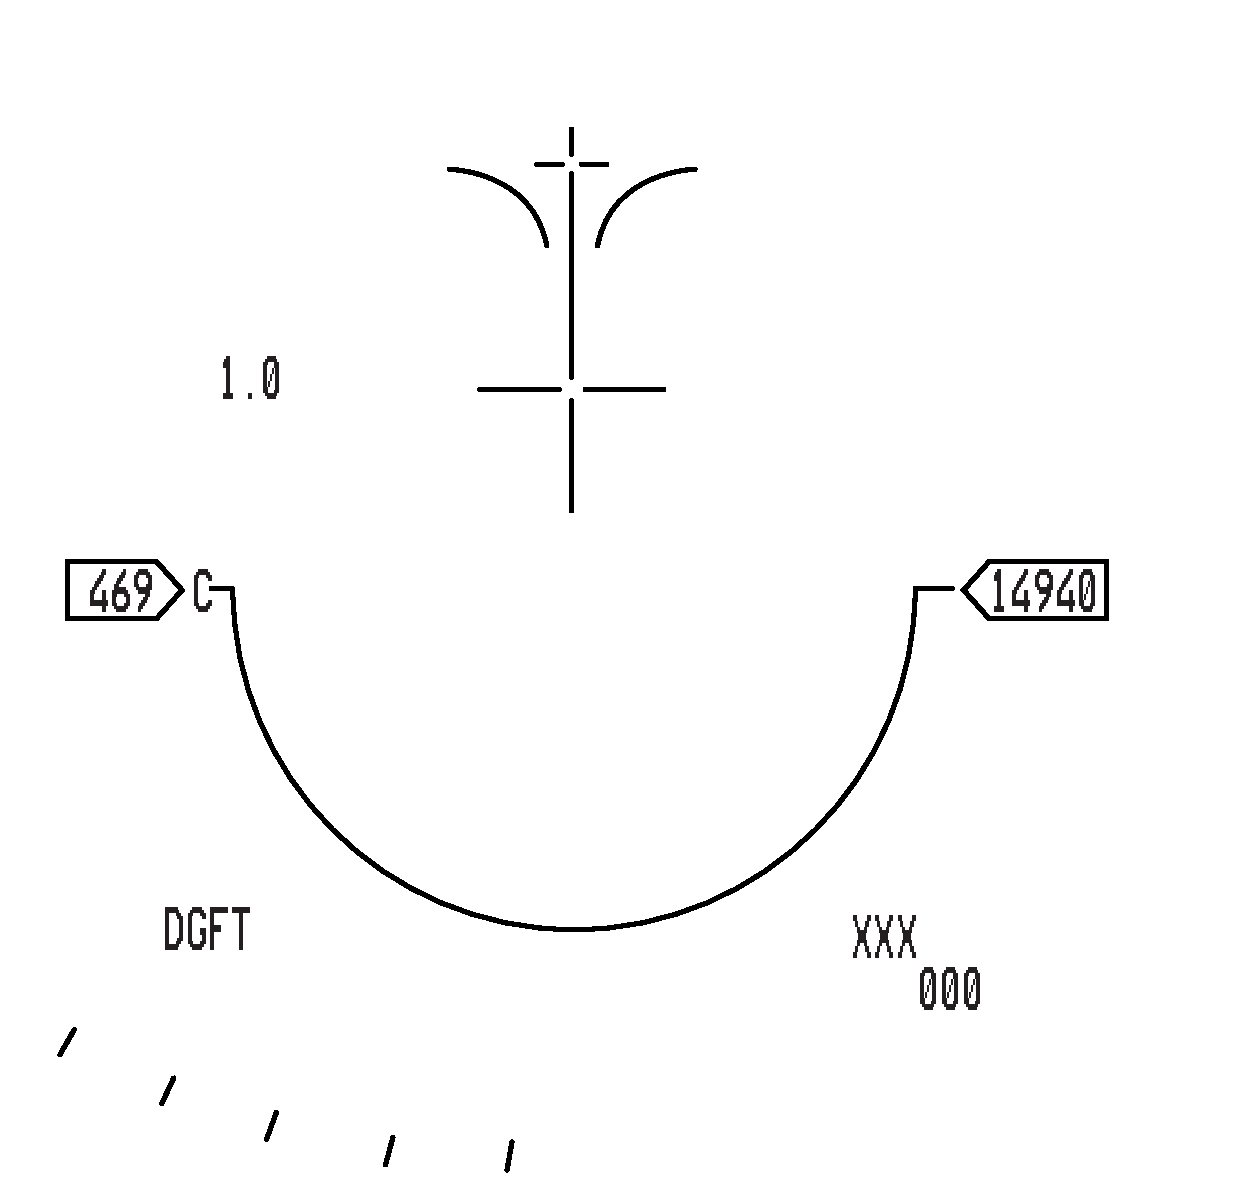
\includegraphics[
                height=75mm,
            ]{hud/acm/bore.pdf}
        };

        % Annotations
        \node[lannot] (bs) at ($(fig.west)+(-2.5mm,34mm)$) {Boresight cross};
        \draw[->, red] (bs.east) -- ++(34mm,0mm) -- ++(4mm,-4mm);

        \node[lannot] (eegs) at ($(fig.west)+(-2.5mm,24mm)$) {EEGS funnel};
        \draw[->, red] (eegs.east) -- ++(32mm,0mm);

        \node[lannot] (acc) at ($(fig.west)+(-2.5mm,13.5mm)$) {Acceleration};
        \draw[->, red] (acc.east) -- ++(16mm,0mm);

        \node[lannot] (cas) at ($(fig.west)+(-2.5mm,0mm)$) {Airspeed \\ {\footnotesize calibrated}};
        \draw[->, red] (cas.east) -- ++(7mm,0mm);

        \node[lannot] (dgft) at ($(fig.west)+(-2.5mm,-15mm)$) {Mode};
        \draw[->, red] (dgft.east) -- ++(9mm,0mm) -- ++(4mm, -4mm);

        \node[lannot] (mgrs) at ($(fig.west)+(-2.5mm,-32mm)$) {MGRS lines};
        \draw[->, red] (mgrs.east) -- ++(10mm,0mm);

        \node[rannot] (bore) at ($(fig.east)+(2.5mm,13mm)$) {Scan zone indicator};
        \draw[->, red] (bore.west) -- ++(-38mm, 0mm);

        \node[rannot] (alt) at ($(fig.east)+(2.5mm,0mm)$) {Altimeter};
        \draw[->, red] (alt.west) -- ++(-12mm, 0mm);

        \node[rannot] (arc) at ($(fig.east)+(2.5mm,-12mm)$) {Attitude arc};
        \draw[->, red] (arc.west) -- ++(-28mm, 0mm);

        \node[rannot] (slant) at ($(fig.east)+(2.5mm,-25.25mm)$) {Target slant range};
        \draw[->, red] (slant.west) -- ++(-20mm, 0mm);
    \end{tikzpicture}
    \caption{ACM HUD Symbology. Shown in BORE submode.}
\end{figure}

\begin{figure}[htbp]
    \centering
    \begin{tikzpicture}[auto, node distance=10mm, x=1mm, y=1mm, very thick, line cap=round,
        >={Latex[round]}
        ]

        \node[draw, rounded corners] (fig) at (0,0) {
            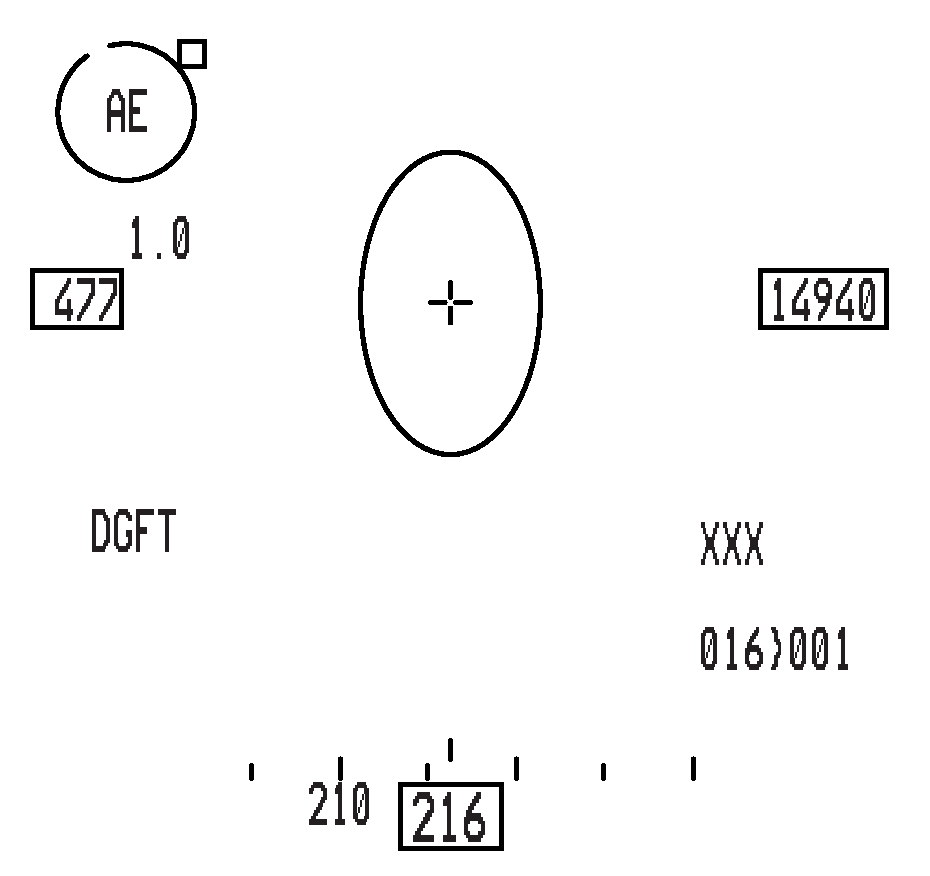
\includegraphics[
                height=60mm,
            ]{hmd/dgft.pdf}
        };

        % Annotations
        \node[lannot] (rwr) at ($(fig.west)+(-2.5mm,22.5mm)$) {RWR};
        \draw[->, red] (rwr.east) -- ++(7mm,0mm);

        \node[lannot] (acc) at ($(fig.west)+(-2.5mm,16.5mm)$) {Acceleration};
        \draw[->, red] (acc.east) -- ++(8mm,0mm) -- ++(4mm, -2mm);

        \node[lannot] (cas) at ($(fig.west)+(-2.5mm,9.5mm)$) {Airspeed};
        \draw[->, red] (cas.east) -- ++(5.5mm,0mm);

        \node[lannot] (cross) at ($(fig.west)+(-2.5mm,2mm)$) {Aiming cross};
        \draw[->, red] (cross.east) -- ++(28mm,0mm) -- ++(5mm,5mm);

        \node[lannot] (dgft) at ($(fig.west)+(-2.5mm,-6.5mm)$) {Mode};
        \draw[->, red] (dgft.east) -- ++(7mm,0mm);

        \node[lannot] (hdg) at ($(fig.west)+(-2.5mm,-26mm)$) {Heading \\ {\footnotesize HMD LOS}};
        \draw[->, red] (hdg.east) -- ++(22mm,0mm);

        \node[rannot] (acq) at ($(fig.east)+(2.5mm,22.5mm)$) {Acquisition circle};
        \draw[->, red] (acq.west) -- ++(-28mm,0mm) -- ++(-4mm,-4mm);

        \node[rannot] (alt) at ($(fig.east)+(2.5mm,9.5mm)$) {Altimeter};
        \draw[->, red] (alt.west) -- ++(-6mm, 0mm);

        \node[rannot] (range) at ($(fig.east)+(2.5mm,-1mm)$) {Target slant range};
        \draw[->, red] (range.west) -- ++(-10mm, 0mm) -- ++(-4mm, -4mm);

        \node[rannot] (stpt) at ($(fig.east)+(2.5mm,-14.5mm)$) {Distance to STPT};
        \draw[->, red] (stpt.west) -- ++(-8mm, 0mm);
    \end{tikzpicture}
    \caption{
        ACM HMD Symbology. 
        Shown in BORE submode. 
        Note that RWR indication is of highest threat 
        with diamond indicating direction of threat 
        and gap indicating current HMD LOS.
    }
\end{figure}

\begin{tcoloritemize}
    \blueitem{HUD Submode}{
    \begin{subitemize}
        \item \textbf{30x20 deg scan} --- slightly larger than HUD
        \item \textbf{Lock Range} --- 10 nm
        \item \textbf{Selected with TMS Right} --- default mode upon ACM selection
        \item \textbf{Default ACM mode} --- but in \textbf{NO RAD} (non-radiating) state
        \item \textbf{Displays}
        \begin{itemize}
            \item \textbf{FCR Format} --- displays \textbf{ACM 20}
            \item \textbf{HUD} --- no special symbology
        \end{itemize}
    \end{subitemize}}
    \blueitem{BORE Submode}{
    \begin{subitemize}
        \item \textbf{Small, 1-beamwidth scan}
        \begin{itemize}
            \item centered 3 deg below gun cross
            \item useful for precisely locking up target
        \end{itemize}
        \item \textbf{Lock Range} --- 20 nm
        \item \textbf{Selected with TMS Forward}
        \item \textbf{Scan slaves to HMD} (if equipped and powered)
        \item \textbf{Displays}
        \begin{itemize}
            \item \textbf{FCR Format} --- displays \textbf{ACM BORE}
            \item \textbf{HUD} --- Boresight Cross at center of radar scan zone
            \item \textbf{HMD} --- Oval centered on HMD aiming cross
        \end{itemize}
    \end{subitemize}}
    \blueitem{Vertical \break Submode}{
    \begin{subitemize}
        \item \textbf{10x60 deg scan}
        \begin{itemize}
            \item centered 23 deg above gun cross
            \item useful during turning engagement to lock target ``across the circle''
        \end{itemize}
        \item \textbf{Lock Range} --- 10 nm
        \item \textbf{Selected with TMS Aft}
        \item \textbf{Displays}
        \begin{itemize}
            \item \textbf{FCR Format} --- displays \textbf{ACM 60}
            \item \textbf{HUD} --- Vertical line
        \end{itemize}
    \end{subitemize}}
    \blueitem{Slewable \break Submode --- WIP}{
    \begin{subitemize}
        \item \textbf{Scan} --- WIP
        \item \textbf{Lock Range} --- WIP
        \item \textbf{Slew} --- \textbf{CURSOR/ENABLE Control}
        \item \textbf{Displays}
        \begin{itemize}
            \item \textbf{FCR Format} --- displays \textbf{ACM SLEW}
            \item \textbf{HUD} --- WIP
        \end{itemize}
    \end{subitemize}}
    \blueitem{NO RAD}{Upon selection of \textbf{ACM} or dropping target lock the radar is placed in non-radiating state}
\end{tcoloritemize}

\marginfigeometry

\subsubsection{HUD / BORE / VERTICAL ACQUISITION}
\begin{checklistenumerate}
    \blueitem{FCR Setup}{
    \marginpar{
        \captionsetup{type=figure}
        \begin{subfigure}[t]{\linewidth}
            \centering
            \begin{tikzpicture}[auto, node distance=10mm, x=1mm, y=1mm, very thick, line cap=round,
                >={Latex[round]}
                ]
    
                \draw[color2, fill=color2!20, dashed, rounded corners]
                (-15, 10) -- (15,10) -- (15,-10) -- (-15,-10) -- cycle;
                
                \node[] (hud) at (0,0) {
                    
\includegraphics[
                        scale=0.25,
                    ]{hud/acm/subfig_hud.pdf}
                };
        
            \end{tikzpicture}
            \caption{HUD}
        \end{subfigure}
        \begin{subfigure}[t]{0.45\linewidth}
            \centering
            \begin{tikzpicture}[auto, node distance=10mm, x=1mm, y=1mm, very thick, line cap=round,
                >={Latex[round]}
                ]
    
                \draw[color2, fill=color2!20, dashed] 
                (0,-3) circle [x radius=4, y radius=6];
                
                \node[] (bore) at (0,0) {
                    
\includegraphics[
                        scale=0.25,
                    ]{hud/acm/subfig_bore.pdf}
                };
        
            \end{tikzpicture}
            \caption{BORE}
        \end{subfigure}
        \begin{subfigure}[t]{0.45\linewidth}
            \centering
            \begin{tikzpicture}[auto, node distance=10mm, x=1mm, y=1mm, very thick, line cap=round,
                >={Latex[round]}
                ]
    
                \draw[color2, fill=color2!20, dashed, rounded corners]
                (-2.5, 30) -- (2.5,30) -- (2.5,-8) -- (-2.5,-8) -- cycle;
                
                \node[] (vert) at (0,0) {
                    
\includegraphics[
                        scale=0.25,
                    ]{hud/acm/subfig_vert.pdf}
                };
        
            \end{tikzpicture}
            \caption{Vertical}
        \end{subfigure}
        \caption{HUD / BORE / VERTICAL Symbology}
    }
    \begin{subenumerate}
        \item \textbf{FCR Switch} \dotfill \textbf{FCR}
        \item \textbf{Desired MFD} \dotfill \textbf{FCR Page}
    \end{subenumerate}}
    \blueitem{Enter ACM}{
    \begin{subenumerate}
        \item \textbf{Dogfight/Missile Override} \dotfill \textbf{DGFT}
        \item \textbf{Radar Mode (OSB 2)} \dotfill verify \textbf{ACM}
    \end{subenumerate}}
    \blueitem{Select ACM Submode}{
    \begin{subitemize}
        \item \textbf{HUD} (default ACM mode) \dotfill \textbf{TMS Right}
        \item \textbf{Bore} \dotfill \textbf{TMS Forward}
        \item \textbf{Vertical} \dotfill \textbf{TMS Aft}
    \end{subitemize}}
    \blueitem{Target Acquisition}{
    \begin{subenumerate}
        \item Maneuver aircraft to place target within selected ACM scan volume 
        \item Wait for automatic transition to STT 
    \end{subenumerate}}
    \blueitem{Target Rejection}{%
    To unlock target
    \begin{subenumerate}
        \item \textbf{TMS} \dotfill \textbf{Aft}
    \end{subenumerate}
    Radar returns to \textbf{HUD} submode in \textbf{NO RAD} 
    }
\end{checklistenumerate}

\subsubsection{HMD ACQUISITION}
\begin{checklistenumerate}
    \blueitem{FCR/MFD Setup}{
    \marginpar{
        \captionsetup{type=figure}
        \centering
        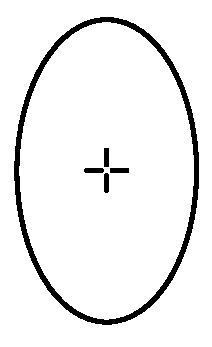
\includegraphics[
            height=25mm,
        ]{hmd/dgft_subfig_bore.pdf}
        \caption{HMD acquisition circle}
    }
    \begin{subenumerate}
        \item \textbf{FCR Switch} \dotfill \textbf{FCR}
        \item \textbf{Desired MFD} \dotfill \textbf{FCR Page}
        \item \textbf{HMD Brightness} \dotfill \textbf{On}
    \end{subenumerate}}
    \blueitem{Enter ACM}{
    \begin{subenumerate}
        \item \textbf{Dogfight/Missile Override} \dotfill \textbf{DGFT}
        \item \textbf{Radar Mode (OSB 2)} \dotfill verify \textbf{ACM}
    \end{subenumerate}}
    \blueitem{Select ACM Bore Submode}{
    \begin{subitemize}
        \item \textbf{Bore} \dotfill \textbf{TMS Forward}
    \end{subitemize}}
    \blueitem{Target Acquisition}{
    \begin{subenumerate}
        \item Maneuver aircraft to place target within 60 deg of nose 
        \item Place target within HMD acquisition circle
        \item Wait for automatic transition to STT 
    \end{subenumerate}}
    \blueitem{Target Rejection}{%
    To unlock target
    \begin{subenumerate}
        \item \textbf{TMS} \dotfill \textbf{Aft}
    \end{subenumerate}
    Radar returns to \textbf{HUD} submode in \textbf{NO RAD} 
    }
\end{checklistenumerate}

\subsubsection{SLEWABLE ACQUISITION --- WIP}

\marginfigrestore

\subsection{STT}
\label{subsec:stt}
\begin{tcoloritemize}
    \blueitem{STT}{
    \textbf{S}ingle \textbf{T}arget \textbf{T}rack
    \begin{subitemize}
        \item \textbf{FCR continually scans one target}
        \begin{itemize}
            \item high update frequency \& precision for weapon guidance
            \item \underline{target RWR will detect STT lock}
        \end{itemize}
        \item \textbf{FCR search ceases during STT lock}
        \item \textbf{Entered by}
        \begin{itemize}
            \item locking bugged target from \textbf{TWS/RWS} with \textbf{TMS Forward}
            \item placing target in search volume of \textbf{ACM} (lock occurs automatically)
        \end{itemize}
        \item \textbf{Exited with TMS Aft} --- returns to search mode
    \end{subitemize}}
    \blueitem{Display}{
    \begin{subitemize}
        \item \textbf{Target state} shown at top of FCR page
        \begin{itemize}
            \item aspect angle 
            \item ground track 
            \item airspeed 
            \item closure rate
        \end{itemize}
    \end{subitemize}}
    \blueitem{NCTR}{
    \textbf{N}on-\textbf{C}ooperative \textbf{T}arget \textbf{R}ecognition
    \begin{subitemize}
        \item \textbf{FCR attempts to identify locked target}
        \begin{itemize}
            \item measures turbine parameters to produce \underline{likely} contact aircraft type
            \item NCTR is only available in STT
        \end{itemize}
        \item \textbf{NCTR imposes additional requirements}
        \begin{itemize}
            \item target must be within 20-25nm
            \item radar must ``see'' compressor/turbine blades
        \end{itemize}
        \item \textbf{Activated with IFF interrogation (TMS Left long)}
        \item \textbf{Hostile NCTR identification counts towards ROE matrix} (combined with IFF return)
    \end{subitemize}}
\end{tcoloritemize}

\begin{figure}[htbp]
    \centering
    \begin{tikzpicture}[auto, node distance=10mm, x=1mm, y=1mm, very thick, line cap=round,
        >={Latex[round]}
        ]
        
        \node[] (mfd) at (0,0) {
            \includegraphics[
                height=100mm,
                page={37},
            ]{F16_apg68_RWS_HomePage&SAM_v6-1.pdf}
        };

        \node[] at (0,-20) {\color{red}\textbf{MISSING ANNOTATIONS}};
    \end{tikzpicture}
    % \fbox{
    % \begin{minipage}[t][75mm][t]{100mm}
    %     \center{\large\textbf{MFD --- FCR --- STT}}
    %     \begin{itemize}
    %         \item Show standard STT lock
    %         \item should clearly mark target state, steering cues, dlz, NCTR
    %     \end{itemize}
    % \end{minipage}
    % }
    \caption{FCR page with STT lock and NCTR ID}
\end{figure}
